\documentclass[reprint,superscriptaddress,floatfix]{revtex4-2}
\usepackage{braket,amsmath,graphicx,color}
\usepackage{hyperref}
\bibliographystyle{apsrev4-1}
\begin{document}

\title{Local metal-insulator transition in a generalised Anderson impurity model}
\author{Abhirup Mukherjee}
\email{am18ip014@iiserkol.ac.in }
\affiliation{Department of Physical Sciences, Indian Institute of Science Education and Research-Kolkata, W.B. 741246, India}
\author{N. S. Vidhyadhiraja}
\email{raja@jncasr.ac.in}
\affiliation{Theoretical Sciences Unit, Jawaharlal Nehru Center for Advanced Scientific Research, Jakkur, Bengaluru 560064, India}
\author{A. Taraphder}
\email{arghya@phy.iitkgp.ernet.in}
\affiliation{Department of Physics, Indian Institute of Technology Kharagpur, Kharagpur 721302, India}
\author{Siddhartha Lal}
\email{slal@iiserkol.ac.in}
\affiliation{Department of Physical Sciences, Indian Institute of Science Education and Research-Kolkata, W.B. 741246, India}

\date{\today}

\begin{abstract}
Lorem ipsum dolor sit amet, consectetur adipiscing elit, sed do eiusmod tempor incididunt ut labore et dolore magna aliqua. Ut enim ad minim veniam, quis nostrud exercitation ullamco laboris nisi ut aliquip ex ea commodo consequat. Duis aute irure dolor in reprehenderit in voluptate velit esse cillum dolore eu fugiat nulla pariatur. Excepteur sint occaecat cupidatat non proident, sunt in culpa qui officia deserunt mollit anim id est laborumLorem ipsum dolor sit amet, consectetur adipiscing elit, sed do eiusmod tempor incididunt ut labore et dolore magna aliqua. Ut enim ad minim veniam, quis nostrud exercitation ullamco laboris nisi ut aliquip ex ea commodo consequat. Duis aute irure dolor in reprehenderit in voluptate velit esse cillum dolore eu fugiat nulla pariatur. Excepteur sint occaecat cupidatat non proident, sunt in culpa qui officia deserunt mollit anim id est laborumLorem ipsum dolor sit amet, consectetur adipiscing elit, sed do eiusmod tempor incididunt ut labore et dolore magna aliqua. Ut enim ad minim veniam, quis nostrud exercitation ullamco laboris nisi ut aliquip ex ea commodo consequat. Duis aute irure dolor in reprehenderit in voluptate velit esse cillum dolore eu fugiat nulla pariatur. Excepteur sint occaecat cupidatat non proident, sunt in culpa qui officia deserunt mollit anim id est laborum
\end{abstract}

\maketitle

%\tableofcontents

\section{Introduction}

Quantum impurity models, owing to their simple construction, have often served as testbeds for analytical and numerical methods, as well as experimental techniques.
They consist of one or more local correlated quantum system(s) coupled with (typically non-interacting) bosonic or fermionic conduction bath channel(s).
Even though the impurity itself is usually simple, the interaction with the bath is what turns it into a correlated many-body problem, and leads to novel emergent phases. Such impurity systems often give rise to interesting phenomena that have far-reaching consequences and require fundamental theoretical breakthroughs in order to understand them.
One of the most well-studied of these is the single-impurity Anderson model~\cite{anderson_1961,anderson_1978} (AIM), consisting of a single impurity site with local correlation \(U\) hybridising with a non-interacting fermionic conduction bath through a coupling \(V\).
The model combines impurity localisation arising from Mott physics~\cite{Mott_1949,vanvleck_1953} and impurity delocalisation arising from virtual resonance with the conduction bath~\cite{friedel_1956}.
In order to obtain its low-energy behaviour, the AIM (along with its \(U \to \infty\) limit, the Kondo model, as well as the \(U \to -\infty\) limit~\cite{schrieffer1966,taraphder_1991}) has been studied using several analytical and numerical techniques like the Coulomb gas approach~\cite{anderson1969exact,anderson1970exact}, perturbative renormalisation group~\cite{anderson1970,haldane1978scaling,jefferson_1977}, numerical renormalisation group (NRG)~\cite{wilson1975,hrk_wilson_1980}, the Bethe ansatz~\cite{andrei_1980,andreiKondoreview,Wiegmann_1981,tsvelickKondoreview}, bosonization~\cite{kotliar_1996,Duki_2011,borda_2008}, functional renormalisation group~\cite{streib_2013} and, most recently, a unitary renormalisation group approach~\cite{anirban_kondo}. 
The general conclusion for the positive \(U\) case at \(T=0\) is that on the particle-hole symmetric (that is, half-filled) line where the holon and doublon impurity levels are degenerate with each other, the impurity local moment is always screened by the conduction bath through enhanced spin-flip scattering at low-energies, leading to a macroscopic singlet ground state and local Fermi liquid gapless excitations~\cite{nozaki2012,mora_2015}; there is no transition to any unscreened phase for a half-filled impurity. The group of conduction electrons that participate in forming the singlet and perform the screening are commonly referred to as the Kondo cloud~\cite{sorensen_erik_affleck_1996,affleck_ian_2001,simon_pascal_2003,martin2010,martin2019}. Because of technological advances, it has become possible to create such Kondo systems and observe this Kondo cloud in quantum dots using scanning tunnelling spectroscopy (STS) and other techniques~\cite{Goldhaber-Gordon1998,Cronenwett1998,Schmid_Weis1998,pustilnik_glazman_2004,Borzenets2020,neel_berndt_2008,Zhao2005}.

Even though the AIM as well as the Kondo model have been successfully solved, they find use as auxiliary models in the dynamical mean-field theory~\cite{kuramoto1987,Cox1988,metzner_volhardt_1989,kotliar1992}(DMFT)-based methods of solving bulk lattice problems.
Once a bulk model is given in terms of some parameters, the workflow of DMFT in solving this model typically involves (i) starting with an AIM (with a non-interacting bath) defined by the bulk parameters, (ii) calculating its self-energy using impurity solvers like exact diagonalisation~\cite{stanescu_2006,capone2007,sakai_2009}, NRG~\cite{bulla_1998,bulla_1999,bulla2001,zitzler_2004}, quantum Monte Carlo~\cite{hirsch1986,rozenberg1997,gull_2011} or density-matrix renormalisation group~\cite{white1992,peschel_1999,garcia2004,schollwock2005,hallberg2006,garcia2007,garcia2007_prb} (DMRG), (iii) equating the bath \(k-\)space self-energy to the impurity self-energy obtained in the previous step, and (iv) restarting the process with a new AIM defined by the new self-energy.
This continues iteratively until the impurity self-energy converges and becomes equal to the bath self-energy.
The results can be shown to become asymptotically exact in the limit of infinite dimensionality \((d=\infty)\).
Improvements, like introducing non-locality in the self-energy, can be introduced by replacing the single impurity with a cluster of multiple impurities~\cite{parcollet_2004,maier_2005,kotliar_rmp_2006,ohashi_2008}. 

One of the primary motivations and applications of DMFT has been the study of the Mott metal-insulator transition (MIT)~\cite{Mott_1949} in the Hubbard model~\cite{gutzwiller_1963,kanamori_1963,hubbard1963electron}.
The Hubbard model is believed to lie at the heart of the high-\(T_c\) problem and has achieved cult status in the field of strongly-correlated electrons because of the array of interesting phases it hosts~\cite{keimer2015quantum,arovas_2022,qin_2022}, ranging from antiferromagnetic long-range order and spin liquids to spin- and charge-density waves and unconventional superconductivity.
The model has been found to be relevant to several materials like the high-\(T_c\) copper oxides~\cite{zhangrice-physrevb.37.3759}, the high-\(T_c\) nickelates~\cite{Kitatani2020} and organic salts~\cite{scriven_2009}.
Using the AIM as the auxiliary model, an MIT was demonstrated in the \(d=\infty\) Hubbard model at zero temperature and half-filling~\cite{zhang_1993}. The transition is seen through the evolution of the real-space local spectral function (schematically shown in Fig.~\ref{spec-func_scheme}), and the behaviour until the transition is very similar to that of the impurity spectral function in the AIM~\cite{hewson1993}.

\begin{figure}[!htb]
	\centering
	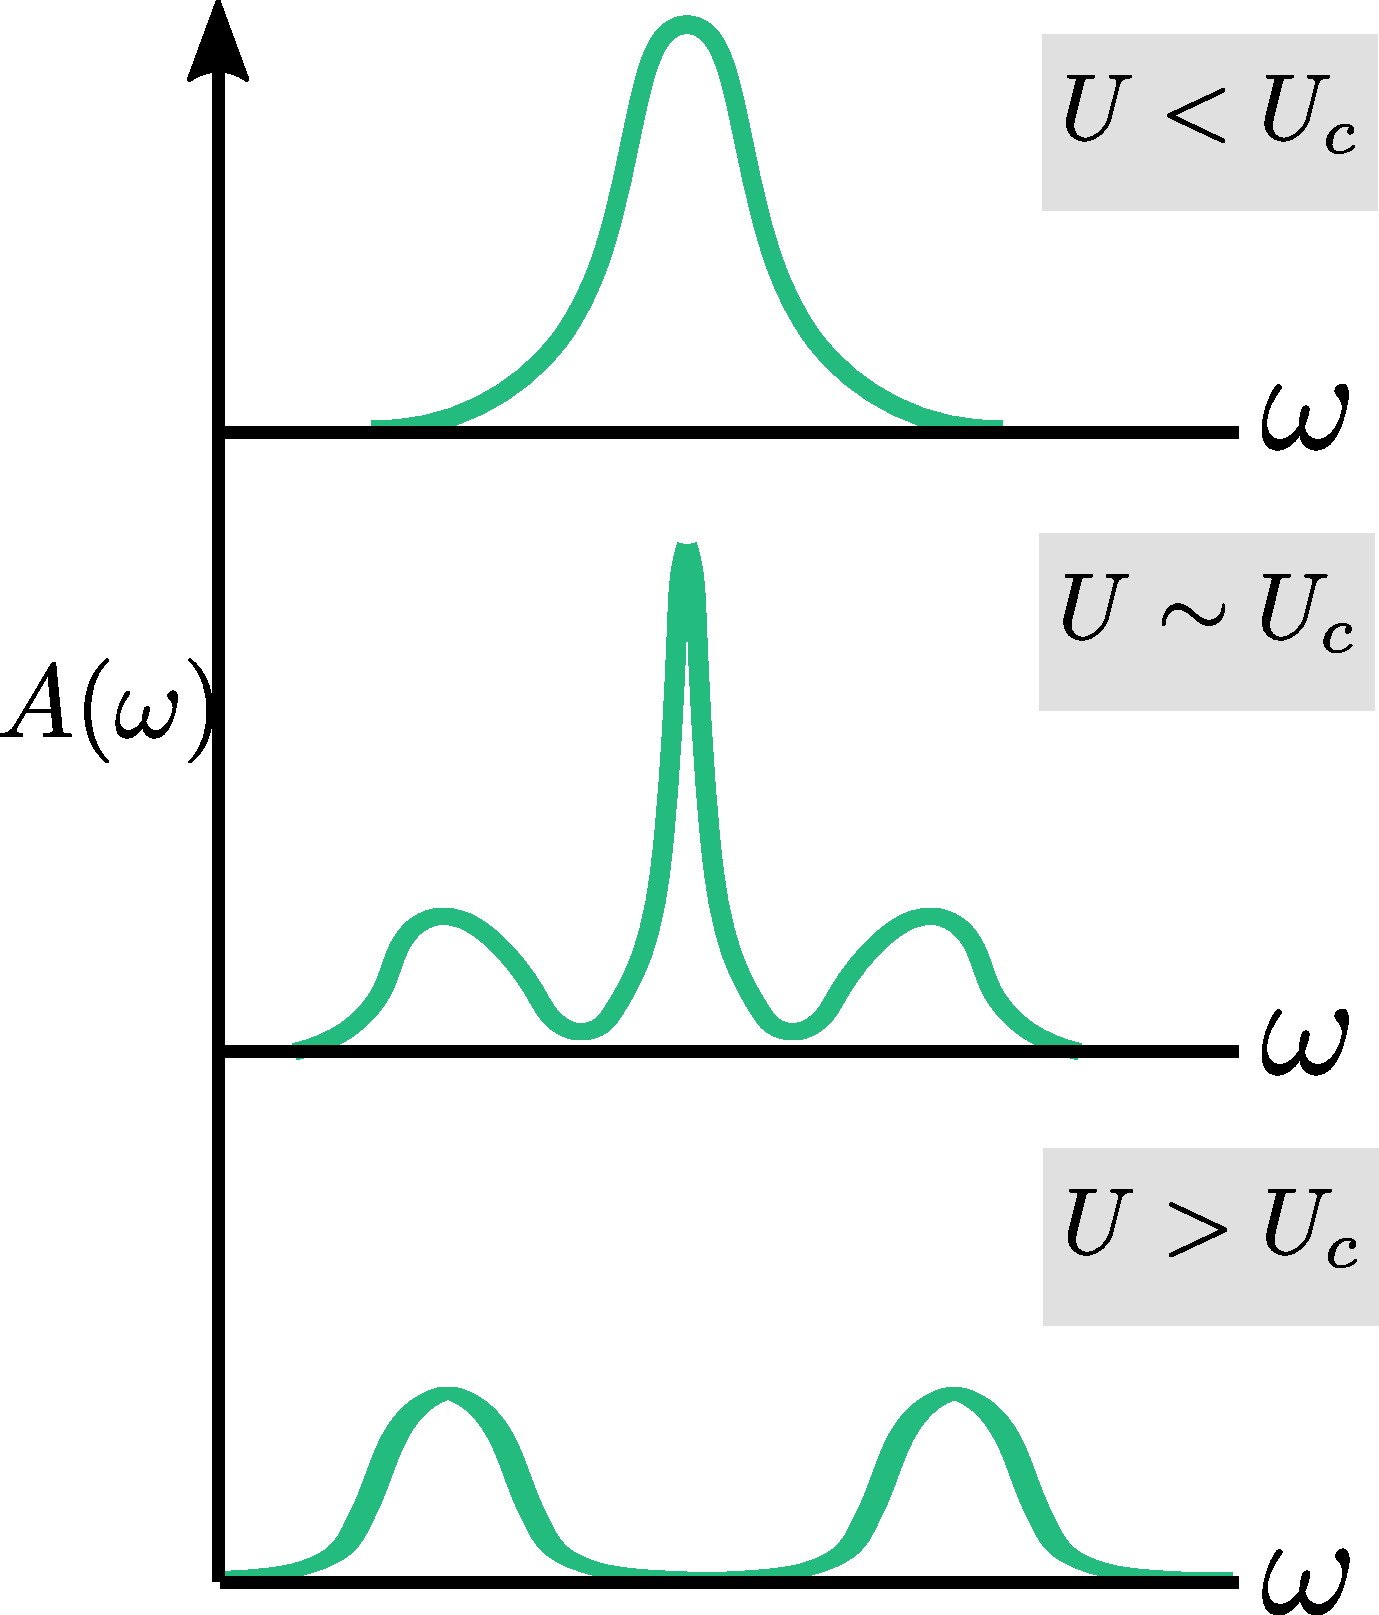
\includegraphics[width=0.35\textwidth]{spec_func.pdf}
	\caption{Schematic description of the evolution of the density of states across the transition~\cite{zhang_1993}.}
	\label{spec-func_scheme}
\end{figure}

Despite the success of DMFT and its cluster-variants, certain points remain to be addressed:
\begin{itemize}
	\item What is the minimal impurity model that can act as an auxiliary model for describing an MIT of the Mott kind?
	\item Having obtained such a minimal model, can we create a formalism that relates (in a transparent and tractable manner) the physics of the bulk to that of the auxiliary model?
	\item Can we then, using such a formulation, try to extract the fluctuations that destabilise the metal and lead to the Mott insulator, as well as study other aspects of the MIT?
\end{itemize}
The reliance of DMFT on the iterative route towards self-consistency means that the impurity auxiliary model gets highly correlated in the process~\cite{held2008}, and no single impurity model can be related to the bulk; for the same reason, it is also not possible, at present, to relate the properties of the auxiliary models to those of the full model. In this {\color{blue}work}, we will focus mostly on the first question, but we will provide hints about the third question as well. Since it has already been established that the AIM does not feature a transition, it is incapable of describing an MIT. This warrants the introduction of additional physics that can destabilise the Kondo cloud.

The paper is structured as follows. Sec.~\ref{def-ham} describes the extended model that we will be studying in this {\color{blue}work}. In Sec.~\ref{method}, we talk about the renormalisation group technique that we employ to study the model and the RG equations obtained from them. Sec.~\ref{phase} lays out the phase diagram and demonstrates the phase transition. Sec.~\ref{eff-ham} gives the effective Hamiltonians in various phases and the zero-bandwidth limits of the ground states. In Sec.~\ref{descr}, we give additional insight into the transition by tracking it via entanglement measures and two-particle correlations. We conclude in Sec.~\ref{concl} with some discussions and possible future directions.

\subsection*{Summary of results}

\begin{itemize}
	\item {\color{blue}Indeed}, we find that on extending the AIM with a spin-exchange interaction \(J\) between the impurity site and the site it is coupled to (zeroth site), and an attractive correlation \(U_b\) on the zeroth site, the enhanced model shows a phase transition under a renormalisation group treatment, at a critical value \(\left(-U_b/J\right)_c=1/4\). 
	\item The ground state can be shown to evolve from a singlet between the impurity and the zeroth site to a decoupled local moment on the impurity, through a correlated state with both spin and charge content.
	\item The transition can be tracked through the variation of the geometric entanglement, which starts from zero in the screened phase and reaches its maximum value of 1 in the local moment phase.
	\item The impurity spectral function shows a three-peak structure at the critical point, similar to the AIM, and develops a gap beyond that.
\end{itemize}
 

\section{The generalised Anderson impurity model}
\label{def-ham}

The impurity models we will work with couple the impurity to a single site in the lattice. We will refer to that specific site as the zeroth site throughout. We recall the Hamiltonian of the Anderson impurity model (AIM) with a half-filled impurity site:
\begin{equation} 
	\mathcal{H} = \frac{- U}{2} \left(\hat n_{d \uparrow} - \hat n_{d \downarrow}\right)^2 + \sum_{\vec k,\sigma} \epsilon_{\vec k} \tau_{\vec k,\sigma} + V\sum_\sigma \left( c^\dagger_{d\sigma}c_{0\sigma} + \text{h.c.}\right)~,
 \end{equation}
where \(\tau_{\vec k,\sigma} \equiv \hat n_{\vec k,\sigma} - 1/2\). Also, \(c_{d\sigma}\) and \(c_{0\sigma}\) are the fermionic annihilation operators of spin \(\sigma\) for the impurity and zeroth sites respectively. \(U\) is the repulsive correlation on the impurity site, and the impurity is at particle-hole symmetry. \(V\) is the momentum-independent hybridisation parameter that couples the impurity with the lattice. We will work with a constant density of states in the bath. 

In order to enhance the Anderson impurity model (AIM), we introduce two extra two-particle interaction terms into the Hamiltonian:
\begin{itemize}
	\item a spin-exchange term \(J \vec{S}_d\cdot\vec{S}_0\) between the impurity spin \(\vec S_d\) and the spin \(\vec S_0\) of the zeroth site 
	\item a local particle-hole symmetric correlation term \(-U_b \hat n_{0 \uparrow} \hat n_{0 \downarrow}\) on the zeroth site
\end{itemize}

With these additional terms, the {\it generalised Anderson impurity model} (henceforth referred to as the GAIM), at particle-hole symmetry, is
\begin{equation}\begin{aligned}
	\label{GIAM-ham}
	\mathcal{H} = -\frac{1}{2}U \left(\hat n_{d \uparrow} - \hat n_{d \downarrow}\right)^2 + \sum_{\vec k,\sigma} \epsilon_{\vec k} \tau_{\vec k,\sigma} + J \vec{S}_d\cdot\vec{S}_0 \\
	+ V\sum_\sigma \left( c^\dagger_{d\sigma}c_{0\sigma} + \text{h.c.}\right) - U_b \hat n_{0 \uparrow} \hat n_{0 \downarrow}
\end{aligned}\end{equation}
All the terms in the Hamiltonian have been depicted schematically in Fig.~\ref{zeromode-bare}.

\begin{figure}[!htb]
	\centering
	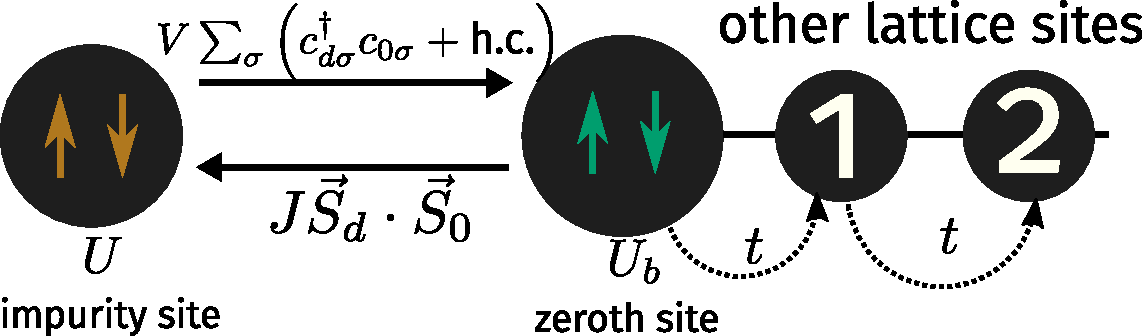
\includegraphics[width=0.45\textwidth]{zeromode_bare.pdf}
	\caption{While we have studied the full model under renormalisation group, often we will turn to a simplified zero-bandwidth version of the model that is obtained by ignoring the kinetic energy part of the Hamiltonian. This zero-bandwidth model is effectively a two site model.}
	\label{zeromode-bare}
\end{figure}

\section{Method and RG Equations}
\label{method}

\subsection{The unitary RG method}
The focus here is on obtaining the low-energy phases of the GAIM. To accomplish this, we perform a renormalisation group analysis of the associated Hamiltonian (eq.~\ref{GIAM-ham}) using the recently developed unitary renormalisation group (URG) method \cite{anirbanurg1,anirbanurg2}. The method has been applied on a wide variety of problems involving quantum spins and correlated fermions, like the Kagome antiferromagnet~\cite{santanukagome}, the 1D~\cite{1dhubjhep} and 2D Hubbard models, with~\cite{anirbanmott2} and without hole doping~\cite{anirbanmott1}, the reduced-BCS pairing hamiltonian~\cite{siddharthacpi}, the single-channel ~\cite{anirban_kondo} as well as multi-channel~\cite{patra_mck} Kondo problems, and other fermionic lattice problems with and without translation invariance~\cite{anirbanurg1,anirbanurg2}. The unitary RG transformations lead to a series of Hamiltonians \(H_{(j)}\) related to the Hamiltonian at the previous step through a unitary transformation; the unitary transformations are defined by the requirement that they remove number fluctuations in high-energy \(k-\)states, thus making the Hamiltonian progressively more block-diagonal in momentum space. The high-energy degrees of freedom that get decoupled in the process become integrals of motion (IOMs) for the Hamiltonian and enter the Hamiltonian only in a purely number-diagonal form.

To be more precise, we first choose a complete basis \(\left\{ \ket{j} \right\} \) and arrange these states from high-energy (UV) to low-energy (IR). Typically we take these states to be the momentum eigenstates \(\left(\ket{j} = \left\{\ket{\vec k \uparrow}, \ket{\vec k \downarrow}\right\}\right)\), and the isoenergetic shells \(\left\{D_{(j)}\right\}\) then define the sequence of states, such that the momenta far away from the Fermi surface (taken to be at higher \(j\) and having \(|D_{(j)}| \gg |\epsilon_F|\)) are taken to be the UV states while those near the Fermi surface (taken to be at lower \(j\) and having \(D_{(j)} \sim \epsilon_F\)) comprise the IR states. This scheme is shown in Fig.~\ref{urg-scheme}.

\begin{figure}[!htb]
	\centering
	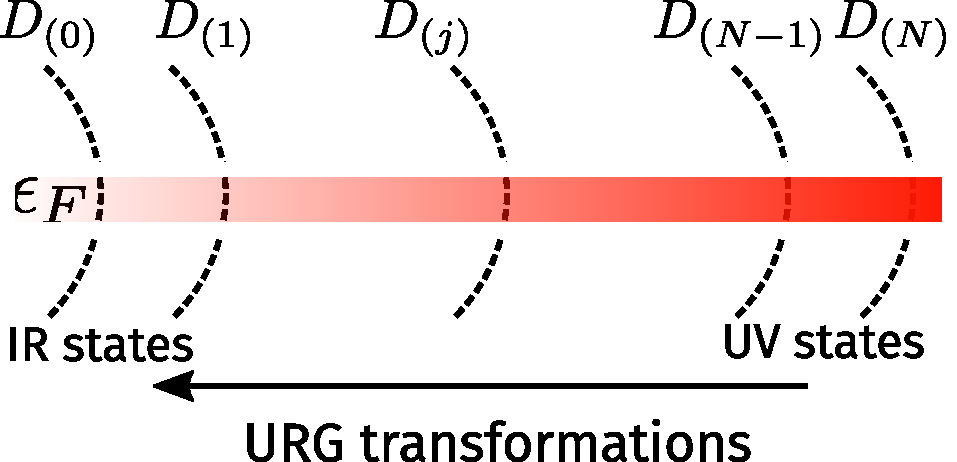
\includegraphics[width=0.45\textwidth]{urg-scheme.pdf}
	\caption{High energy - low energy scheme defined and used in the URG method. The states away from the Fermi surface form the UV subspace and are decoupled first, leading to a Hamiltonian which is more block-diagonal and comprised of only the IR states near the Fermi surface.}
	\label{urg-scheme}
\end{figure}

At a given RG step \(j\), the Hamiltonian \(H_{(j)}\) involves number fluctuations between the \(k-\)states that have energies lower than \(D_{(j+1)}\). So the most energetic states that are still non-trivially present in \(H_{(j)}\) are those on the energy contour \(D_{(j)}\), and the Hamiltonian \(H_{(j)}\) will, in general, not conserve the number of particles in this energy (or momentum) state: \(\left[H_{(j)}, \hat n_{j}\right] \neq 0\). The unitary transformation \(U_{(j)}\) is then defined so as to remove this number fluctuation at the next RG step~\cite{anirbanurg1,anirbanurg2}:
\begin{equation}\begin{aligned}
	H_{(j-1)} = U_{(j)} H_{(j)} U^\dagger_{(j)}~, ~\left[H_{(j-1)}, \hat n_{j}\right] =0~.
\end{aligned}\end{equation}

The unitary transformations can be expressed in terms of a generator \(\eta_{(j)}\) that has fermionic algebra~\cite{anirbanurg1,anirbanurg2}:
\begin{equation}\begin{aligned}
	U_{(j)} = \frac{1}{\sqrt 2}\left(1 + \eta_{(j)} - \eta_{(j)}^\dagger\right)~,~ \quad\left\{ \eta_{(j)},\eta_{(j)}^\dagger \right\}_\pm = 1~,
\end{aligned}\end{equation}
where \(\left\{A,B\right\}_\pm = AB \pm BA\). The generator itself is given by the expression~\cite{anirbanurg1,anirbanurg2}
\begin{equation}\begin{aligned}
	\eta^\dagger_{(j)} = \frac{1}{\hat \omega_{(j)} - \text{Tr}\left(H_{(j)} \hat n_{j}\right) } c^\dagger_{j} \text{Tr}\left(H_{(j)}c_{j}\right)~.
\end{aligned}\end{equation}
The important operator \(\hat \omega_{(j)}\) originates from the quantum fluctuations that exist in the problem because of the non-commutation of the kinetic energy terms and the interaction terms in the Hamiltonian:
\begin{equation}\begin{aligned}
	\hat \omega_{(j)} = H_{(j-1)} - H^i_{(j)}~.
\end{aligned}\end{equation}
\(H^i_{(j)}\) is the part of \(H_{(j)}\) that commutes with \(\hat n_j\) but does {\it not} commute with at least one \(\hat n_l\) for \(l < j\). The RG flow continues up to energy \(D^*\), where a fixed point is reached from the vanishing of the RG function. 

\subsection{URG equations for the GAIM}

The derivation of the RG equations for the generalised Anderson impurity model (GAIM) Hamiltonian is shown in the appendix. We provide below the RG equations for a given quantum fluctuation scale \(\omega\):
\begin{gather}
	\Delta U_b = 0~,\\
	\Delta U = 4V^2 n_j\left(\frac{1}{d_1} - \frac{1}{d_0}\right) - n_j\frac{J^2}{d_2}~,\\
	\Delta V = -\frac{3n_j V}{8}\left[J\left(\frac{1}{d_2} + \frac{1}{d_1}\right) +  \frac{4U_b}{3}\sum_{i=1}^4 \frac{1}{d_i}\right]~,\\
	\Delta J = -\frac{n_j J\left(J + 4U_b\right)}{d_2}~.
\end{gather}
The denominators \(d_i\) used in these equations are given by
\begin{gather}
	d_0 = \omega - \frac{D}{2} + \frac{U_b}{2} - \frac{U}{2}~,d_2 = \omega - \frac{D}{2} + \frac{U_b}{2} + \frac{J}{4}~,\\
	d_1 = \omega - \frac{D}{2} + \frac{U_b}{2} + \frac{U}{2} + \frac{J}{4}~,d_3 = \omega - \frac{D}{2} + \frac{U_b}{2}~.
\end{gather}
The symbols used in the RG equations have the following meanings: \(\Delta U\) represents the renormalisation in the coupling \(U\) in going from the \(j^\text{th}\) Hamiltonian to the \(\left( j-1 \right) ^\text{th}\) Hamiltonian by decoupling the isoenergetic shell at energy \(D_{(j)}\). \(n_j\) is the number of electronic states on the shell \(D_{(j)}\).

We will discuss the consequences of these RG equations in the next sections, but we clarify here that the labels \(U_0,J_0,V_0\) that might occur in the figures or elsewhere in the text represent the bare values of the associated couplings \(U,J\) and \(V\). We also point out here that throughout the upcoming results, the bare value of \(U_b\) is set to the negative of the bare value of \(U_0\): \(U_b = -U_0/10\). This means that whenever we vary \(U_0\) along the axis of a plot, we are simultaneous varying \(U_b\). The reason for choosing the negative sign of \(U_b\) will be clarified in the next section.

\section{RG flows and phase diagram}
\label{phase}

We start the discussion on the nature of the RG flows by noting that the bath correlation \(U_b\) is marginal, and the spin-exchange coupling \(J\) has a critical point \(\left( \Delta J = 0 \right) \) at \(r \equiv -U_b/J = 1/4 \equiv r_c\). We will look at the RG flows of the couplings \(U,V\) and \(J\) on both sides of this critical point by tuning the ratio \(r\) across the critical value \(r_c\), and see what phases they lead to. We will work in the regime of quantum fluctuations where all the denominators are negative: \(d_i < 0 ~\forall~i\). Before we start, note that:
\begin{itemize}
	\item Since \(J\) is positive, this means that we can capture both relevant and irrelevant RG flows of \(J\) by keeping \(U_b\) negative. \(U_b\) is found to be marginal under the RG transformation, and we set \(U_b\) to \(-U_0/10\) hereafter.
	\item The critical point has been chosen from the RG equation of \(J\) and not of \(V\); this is because, the RG irrelevance of \(J\) is sufficient to make \(V\) irrelevant as well, and on the other hand, the RG relevance of \(J\) is sufficient to screen the impurity.
\end{itemize}
  
\begin{figure}[!htb]
	\centering
	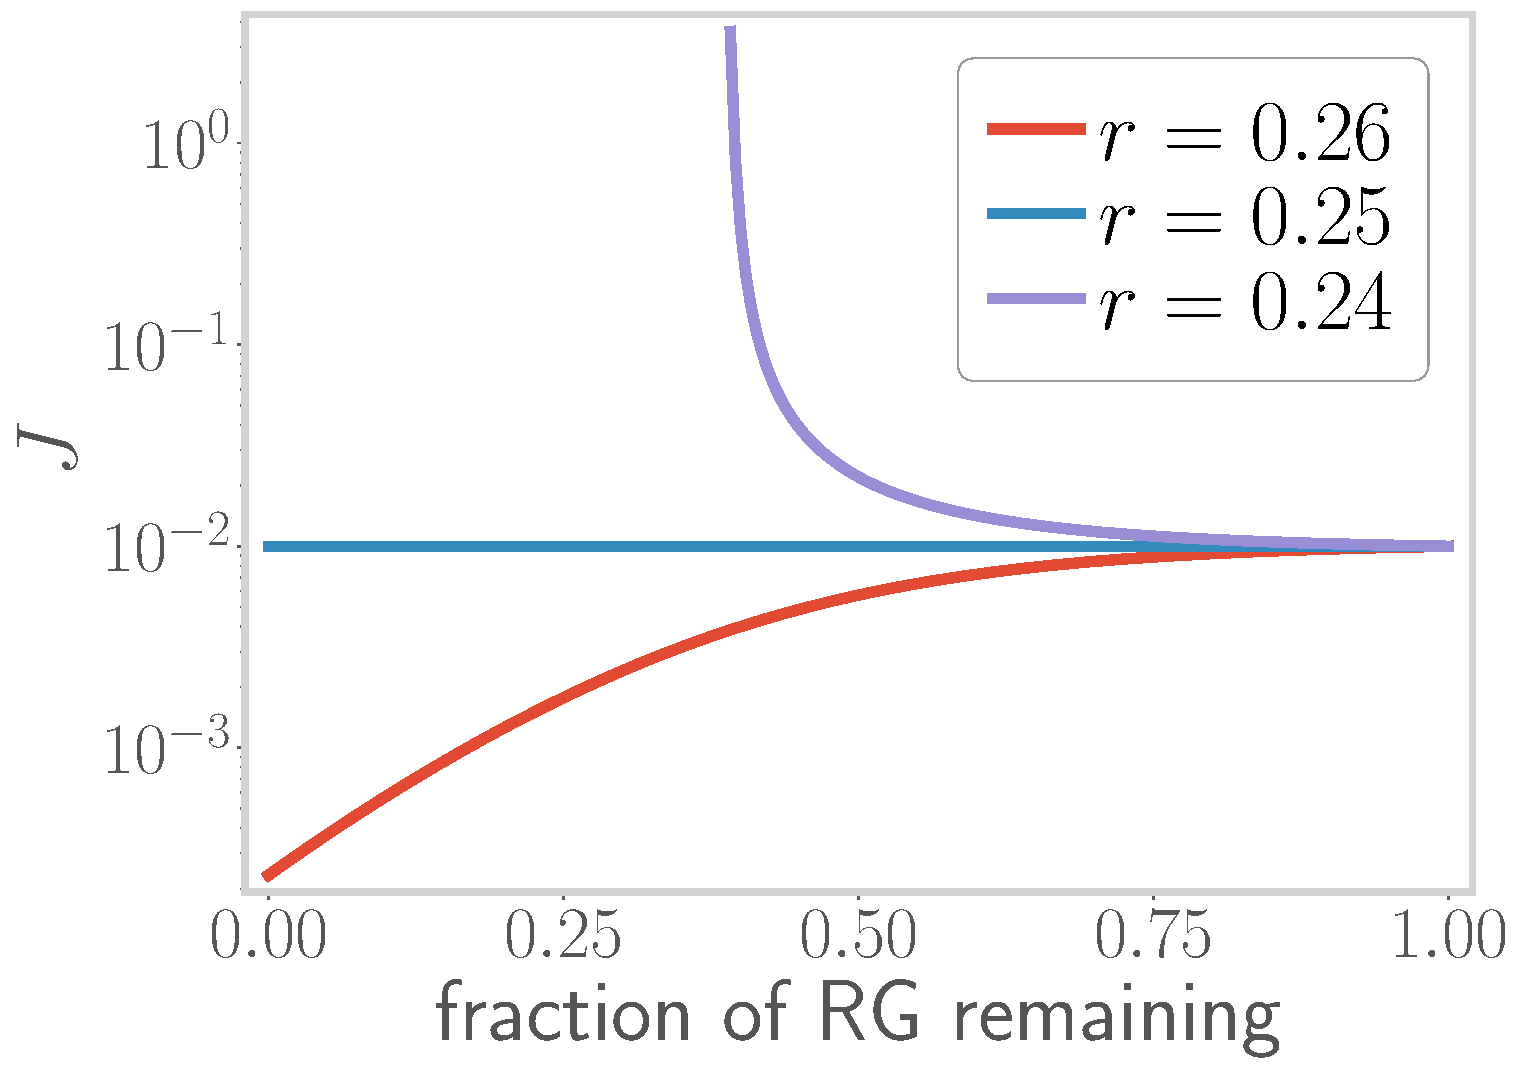
\includegraphics[width=0.48\textwidth]{J_Ub.pdf}
	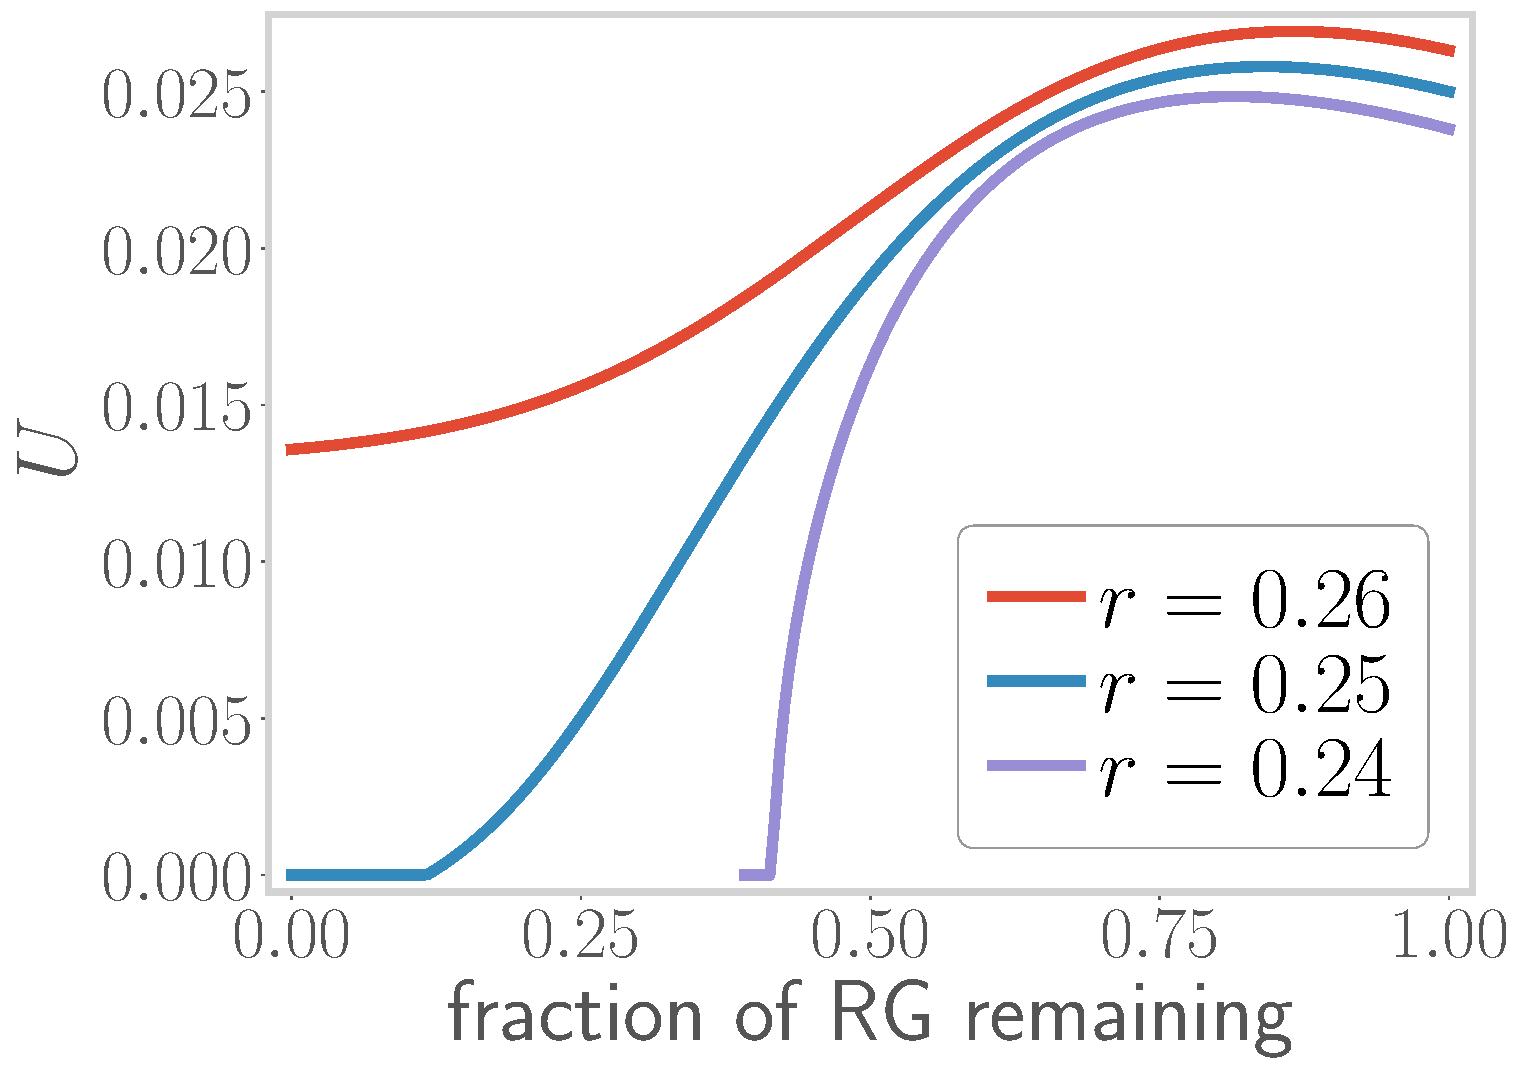
\includegraphics[width=0.48\textwidth]{U_Ub.pdf}
	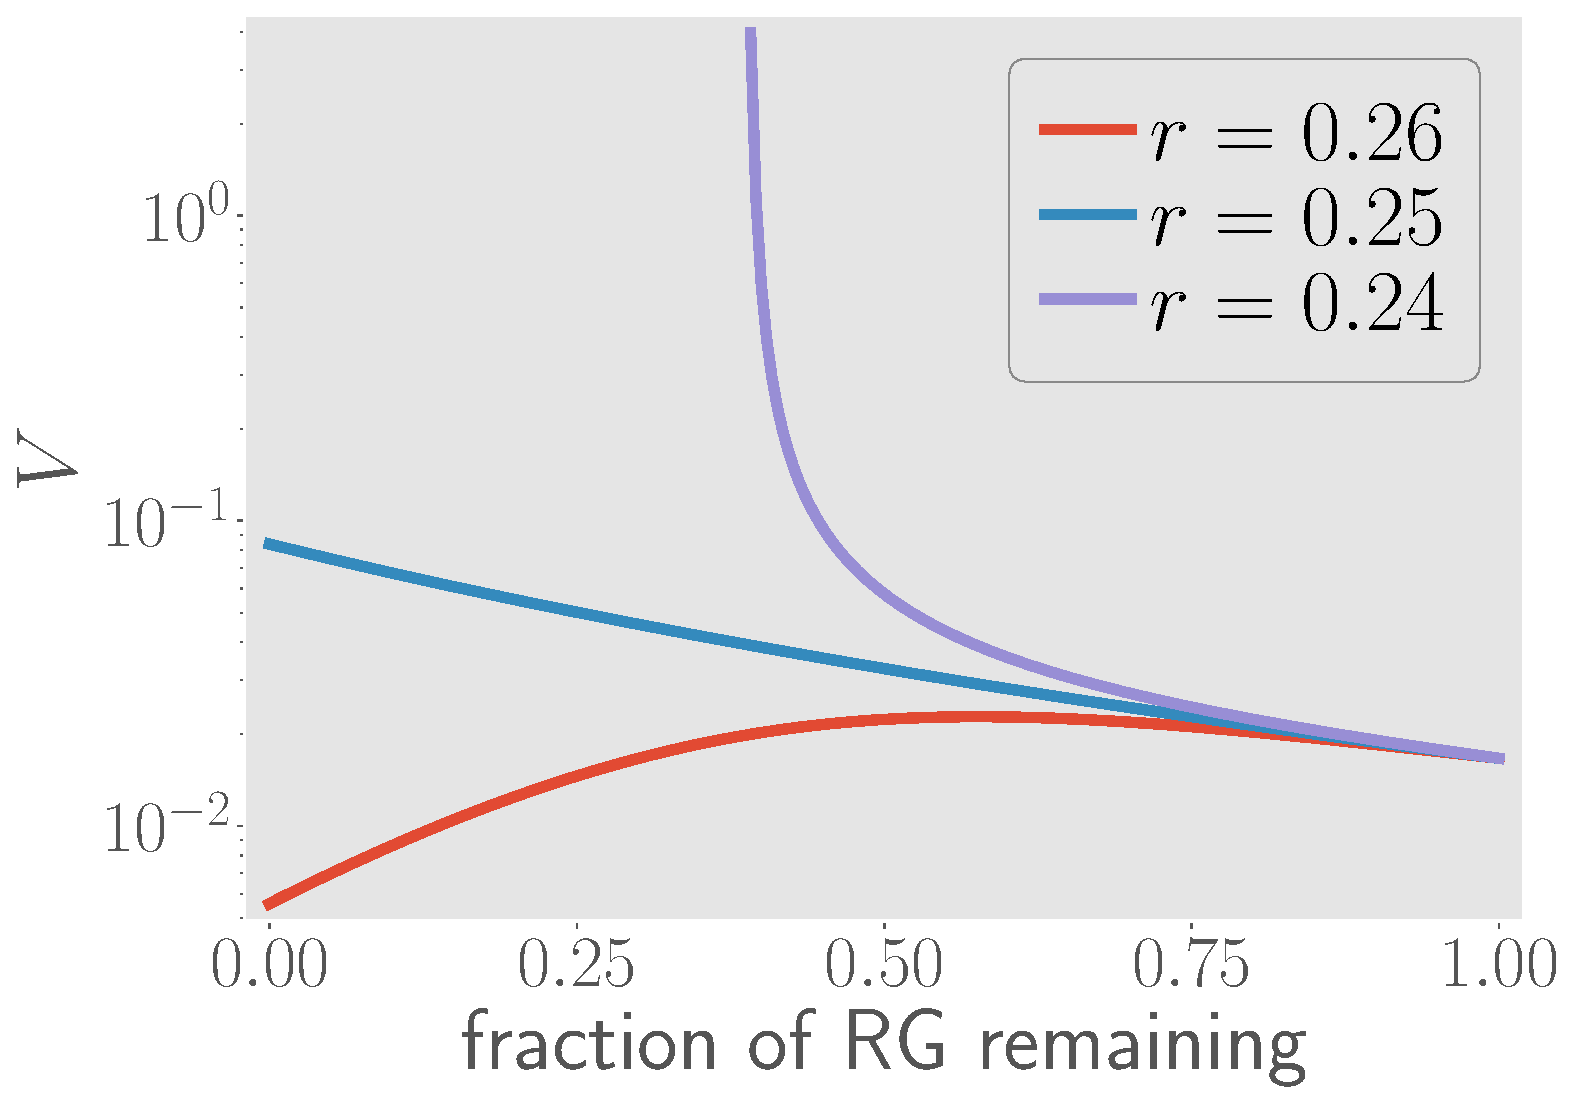
\includegraphics[width=0.48\textwidth]{V_Ub.pdf}
	\caption{Variation of couplings \(U,V\) and \(J\) along the RG transformations, for three values of the transition-tuning ratio \(r\). x-axis represents the RG steps, the rightmost point is the first RG step and leftmost point is the final RG step. The values of the bare couplings are given in the title. All values are in units of the half-bandwidth \(D_0\), which is chosen to be 10. The blue curves represent the flows for \(r > r_c\), where \(J\) is relevant. The purple curves represent the RG flows for \(r < r_c\), where \(J\) is irrelevant. The red curves are exactly at the critical point \(r = r_c\), where \(J\) is marginal.}
	\label{rg-flow}
\end{figure}

\subsection{RG flows for \(r < r_c\)}

In this regime, \(J\) is relevant and flows to large positive values. It is also easy to deduce from its RG equation that \(V\) is also relevant. \(U\) is more non-trivial, because its RG equation involves both \(V\) and \(J\). Nevertheless, the RG equations were solved numerically with bare values of the couplings and the bandwidth, and it was found that while \(V\) and \(J\) are relevant, \(U\) is irrelevant. These findings are shown in the blue curves of Fig.~\ref{rg-flow}. The fixed point values can be summarised as:
\begin{equation}\begin{aligned}
	U^* = 0, ~ ~ ~ ~ V^* \gg 1, ~ ~ ~ ~ J^* \gg 1, ~ ~ ~ ~ U_b \sim \mathcal{O}(1)
\end{aligned}\end{equation}


\subsection{RG flows for \(r > r_c\)}

The RG \(\beta\)-function function for \(J\) changes sign as \(r\) grows greater than \(r_c\) upon tuning \(U_b\) to less than \(-J_0/4\), and \(J\) becomes irrelevant. As for \(V\), note that in the RG equation for \(V\), it is \(J\) that drives \(V\) to be relevant while \(U_b\) drives \(V\) to irrelevance; if \(J\) itself is irrelevant, then \(\Delta V\) will be dominated by \(U_b\) and \(V\) will be ultimately irrelevant. The behaviour of \(U\) is again non-trivial and analytically not tractable, so we solve the RG equations numerically. It turns out that although \(U\) is slightly irrelevant, it saturates to an appreciable value near the fixed point. These RG flows are shown in the purple curves of Fig.~\ref{rg-flow}. The fixed point values in this regime can be summarised as:
\begin{equation}\begin{aligned}
	U^* \sim \mathcal{O}(1), ~ ~ ~ ~ V^* =0, ~ ~ ~ ~ J^* =0, ~ ~ ~ ~ U_b \sim \mathcal{O}(1)
\end{aligned}\end{equation}


\subsection{Phase diagram: impurity phase transition}

The low-energy RG phase diagram is obtained by solving the RG equations for ranges of couplings, and is shown in Fig.~\ref{phase-diag}. There are four distinct phases in the space of couplings \(U_0 \text{ vs } J_0\), with \(U_b\) constrained at \(-U_0/10\) and \(V_0\) set to \(2J_0\). The red phase (phase A in the legend) is composed of those Hamiltonians which lead to RG relevant \(V,J\) and RG irrelevant \(U\). In other words, this is the phase where the impurity moment is screened by the conduction electrons. This is the low-energy phase of the AIM that has \(U\) and \(V\). The blue phase (phase B in the legend) consists of those Hamiltonians which produce irrelevant \(J,V\) and a relevant \(U\); here, the conduction electrons fail to screen the impurity and a residual local moment survives on the impurity at low energies. The yellow phase (phase C in the legend) lies in between these two phases, and is defined by non-negligible \(V^*, U^*\) but zero \(J^*\). In this phase, the impurity still gets screened, but there is more charge content on the impurity site compared to phase B. On going to the thermodynamic limit by increasing the bandwidth \(D_0\), this light green phase disappears. The gray phase (phase D in the legend) is a ``dead" phase where \(U,V,J\) are all RG irrelevant. The various phases are summarised in table.~\ref{summary-phases}.

The black line in Fig.~\ref{phase-diag} represents a line of critical points \(U_b = J_0\), and separates the two major phases of the impurity. Such a {\it phase transition} between the screened impurity and the local moment phases is absent in the AIM without the attractive correlation \(U_b\). In fact, only the purple screened phase is adiabatically connected the AIM.

\begin{table}[!htb]
\centering
\begin{tabular}{|c|c|c|}
\hline
phase & RG flow & fixed point \\ 
\hline
A & \(\Delta U <0, ~ ~ \Delta J,\Delta V>0\) & \(U^* \ll V^* \ll J^*\) \\ 
B &  \(\Delta U > 0, ~ ~ \Delta J,\Delta V<0\) & \(U^* \gg 1, ~ ~V^*, J^* = 0\)\\
C &  \(\Delta U, \Delta J < 0,~ ~\Delta V>0\) & \(J^* < U^* \ll V^*\) \\
D &  \(\Delta U, \Delta J,\Delta V < 0\) & \(U^*, V^*, J^* = 0\) \\
\hline
\end{tabular}
\caption{Summary of the various fixed point phases}
\label{summary-phases}
\end{table}

\begin{figure}[!htb]
	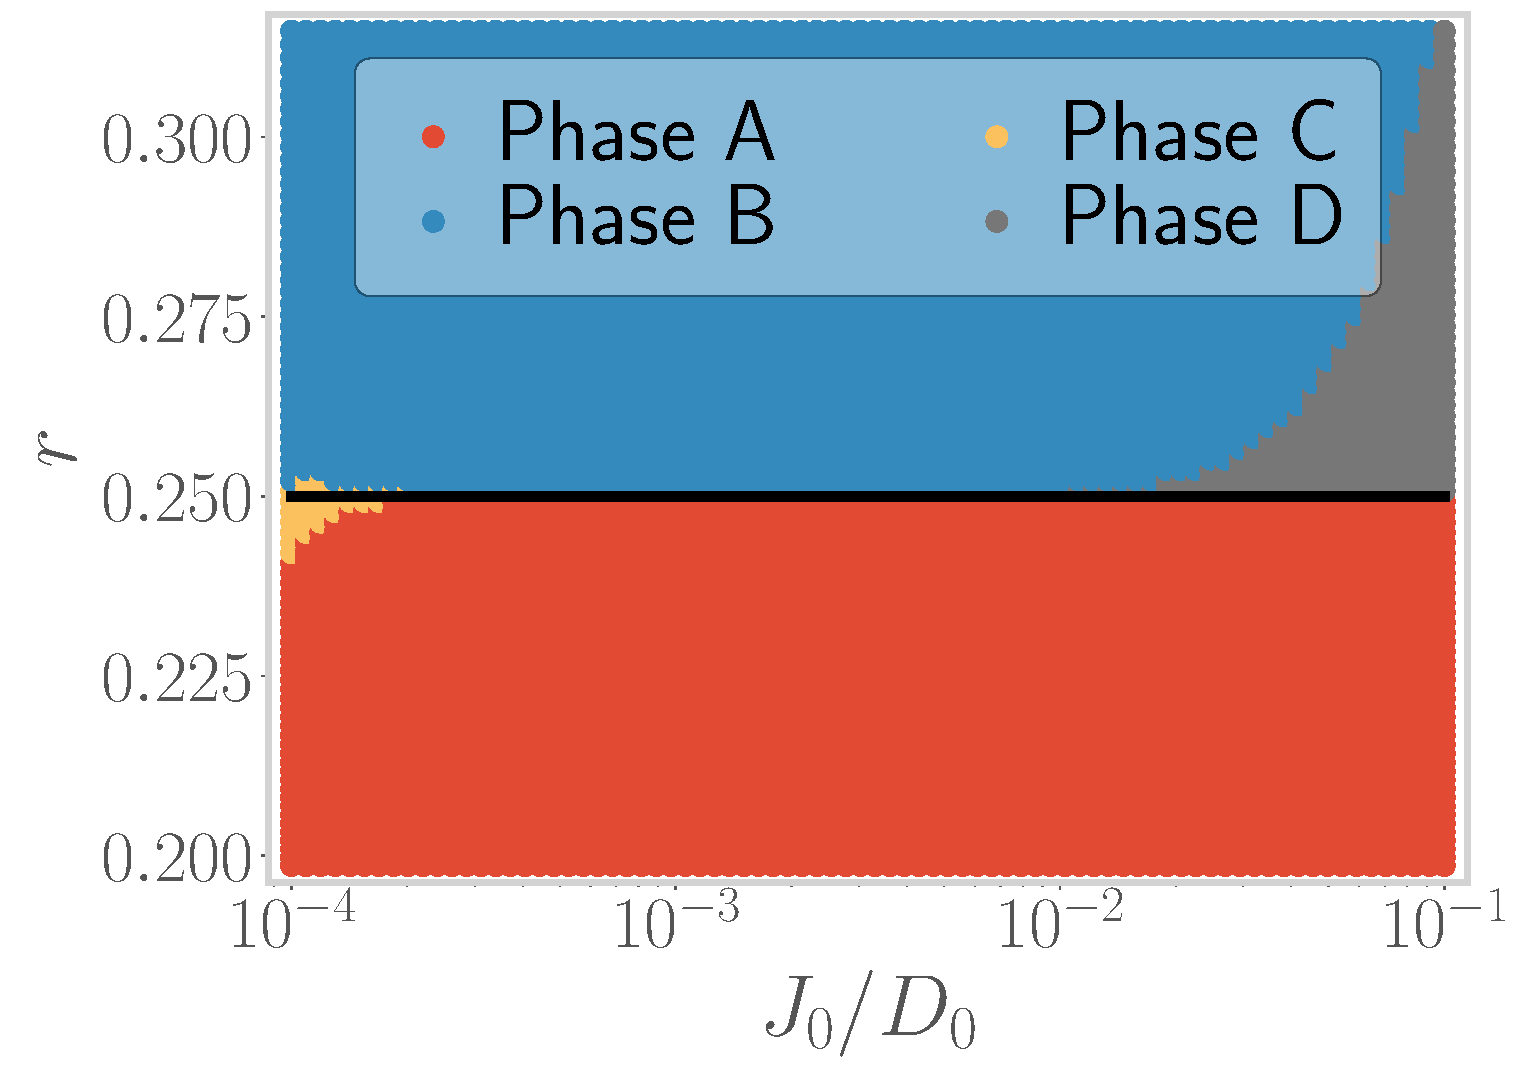
\includegraphics[width=0.48\textwidth]{phase-map-MIT.pdf}
	\caption{Phase diagram of the GAIM, in the space of couplings \(U_0\) and \(J_0\). \(U_b\) is set to \(-U_0/10\) and \(V_0\) is set to \(2J_0\). The various phases \(A\) through \(D\) are characterised in the text.}
	\label{phase-diag}
\end{figure}

\subsection{Growth of charge isospin fluctuations in the bath}
The low-energy phase of the AIM is characterised by enhanced spin-fluctuation \(\left<S_d^+S_0^- + \text{h.c.}\right>\); these fluctuations arise from the Kondo cloud and they serve to screen the local moment. For the system to undergo a transition into an unscreened regime, these fluctuations must get replaced by those of a different kind. This is shown in Fig.~\ref{pair_fluc}, where we plot not only the spin fluctuations mentioned, but also two-particle charge fluctuations \(\left<c^\dagger_{\vec k \uparrow} c^\dagger_{\vec k \downarrow} c_{\vec k^\prime \uparrow} c_{\vec k^\prime \downarrow}\right>\) in the bath that transfer holons and doublons across \(k-\)states. We find that while the former decrease towards the transition, the latter pick up; the spin-fluctuations are getting replaced by the charge fluctuations. This is substantiated by the inset of the same figure, which shows the behaviour of these fluctuations for a larger range across the transition. While the spin-fluctuations vanish beyond the transition, the charge fluctuations undergo an abrupt increase.

{\color{blue}The death of the spin-fluctuations and the simultaneous growth in the charge fluctuations can be attributed to the presence of the attractive correlation term \(U_b\) in the Hamiltonian. Indeed, \(c^\dagger_{\vec k \uparrow} c^\dagger_{\vec k \downarrow} c_{\vec k^\prime \uparrow} c_{\vec k^\prime \downarrow}\) is just the \(k-\)space Fourier transform of the \(U_b\) term. The presence of such terms force the conduction bath to shift spectral weight from the spin sector to the charge sector, destabilising the singlet ground state in the process.}

\begin{figure}[!htb]
	\centering
	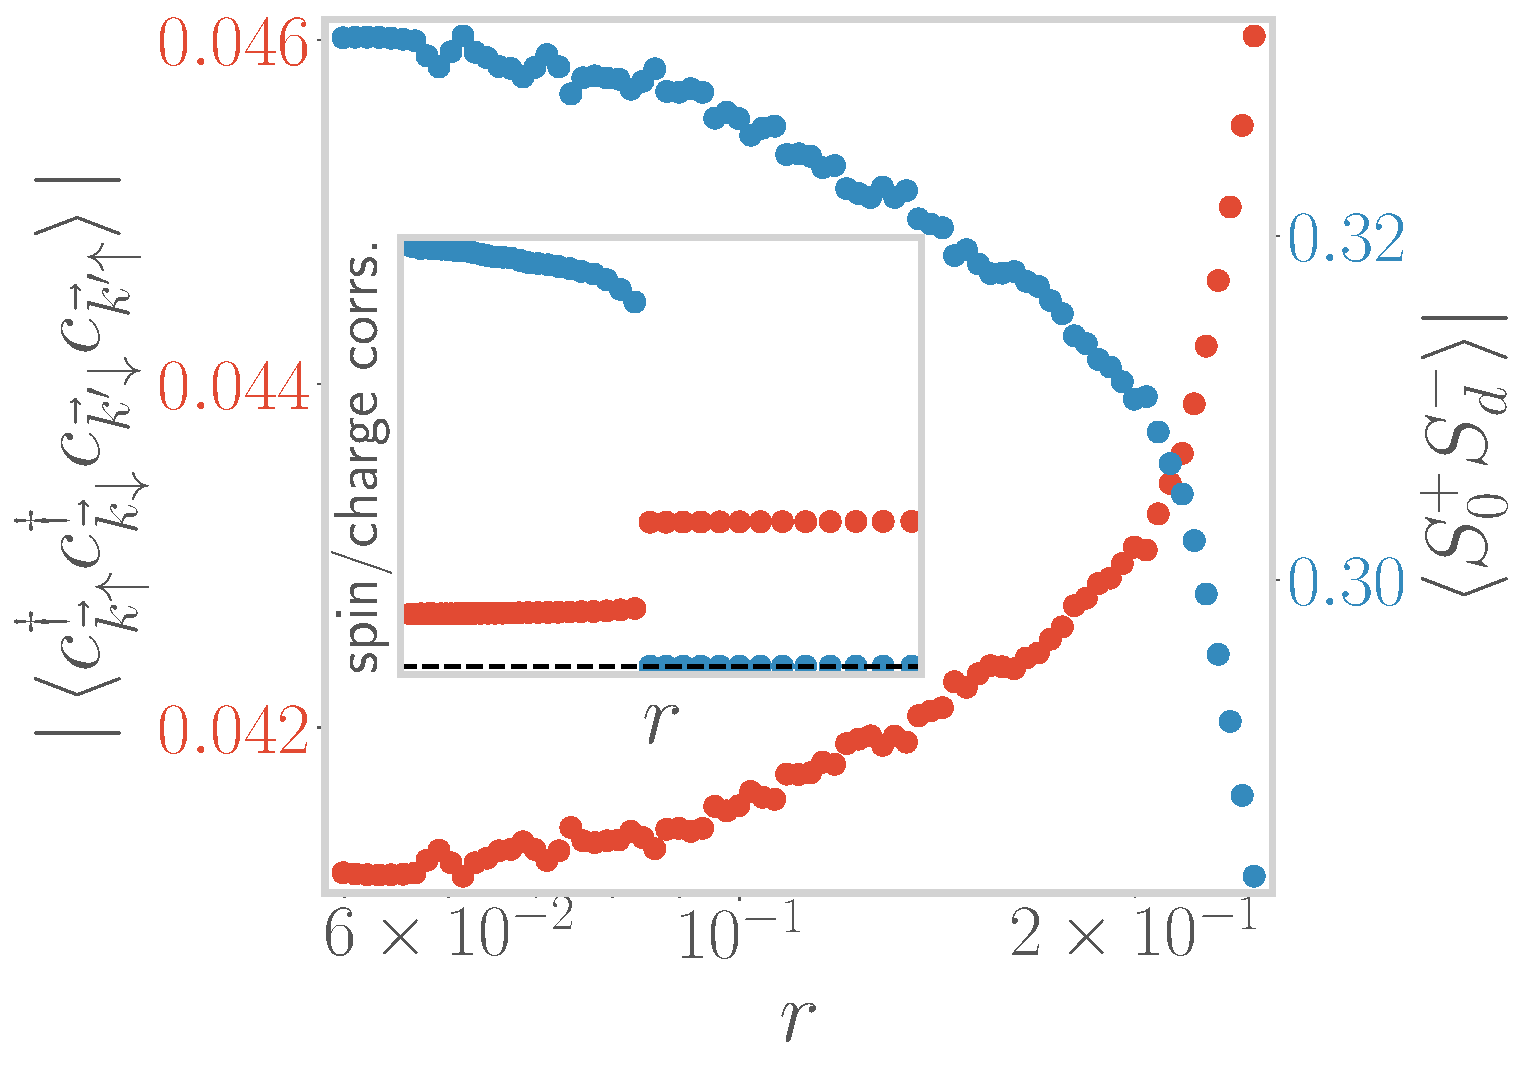
\includegraphics[width=0.49\textwidth]{odlro.pdf}
	\caption{Growth in the pair-fluctuation terms \(c^\dagger_{k \uparrow}c^\dagger_{k \downarrow} c_{k^\prime \downarrow}c_{k^\prime \uparrow}\), as \(r \to 0.25\). This comes at the cost of the spin-flip fluctuations \(S_d^+ S_0^- + \text{h.c.}\), which decrease towards the transition. The inset plots the same quantities but for a larger range of \(r\), and the pair fluctuations are seen to pick up abruptly after the transition while the spin fluctuations vanish.}
	\label{pair_fluc}
\end{figure}

\section{Low-energy effective Hamiltonian and the ground state}
\label{eff-ham}

The RG fixed point Hamiltonian describes the low-energy phase of the system. In general, if the RG fixed point is reached at an energy scale \(D^*\), the fixed point Hamiltonian \(\mathcal{H}^*\) is obtained simply from the fixed point values of the couplings, and by noting that the states above \(D^*\) are now part of the IOMs:
\begin{equation}\begin{aligned}
	\mathcal{H}^* = -\frac{1}{2}U^*\left(\hat n_{d \uparrow} - \hat n_{d \downarrow}\right)^2 + \sum_{\sigma,\vec k:|\epsilon_{\vec k}| < D^*} \epsilon_{\vec k} \tau_{\vec k,\sigma} - U_b^* \hat n_{0 \uparrow} \hat n_{0 \downarrow} \\
	+ V^*\sum_\sigma \left( c^\dagger_{d\sigma}c_{0\sigma} + \text{h.c.}\right) + J^* \vec{S}_d\cdot\vec{S}_0
\end{aligned}\end{equation}

\subsection{Screened regime}
\(U\) is irrelevant in this regime. Moreover, as we go towards the thermodynamic limit by increasing the bandwidth \(D_0\), we find that \(J^* \gg V^*\) (see Fig.~\ref{J_bandwidth}), and the fixed point Hamiltonian is determined purely by the spin-exchange part; combining this with the local bath correlation \(U_b\) that is marginal then gives the low-energy Hamiltonian for the screened regime:
\begin{equation}
	H_\text{eff}^\text{sc} = J^* \vec{S}_d\cdot\vec{S}_0 - U_b \hat n_{0 \uparrow} \hat n_{0 \downarrow} + \sum_{\sigma,\vec k:|\epsilon_{\vec k}| < D^*} \epsilon_{\vec k} \tau_{\vec k,\sigma}
\end{equation}

\begin{figure}[!htb]
	\centering
	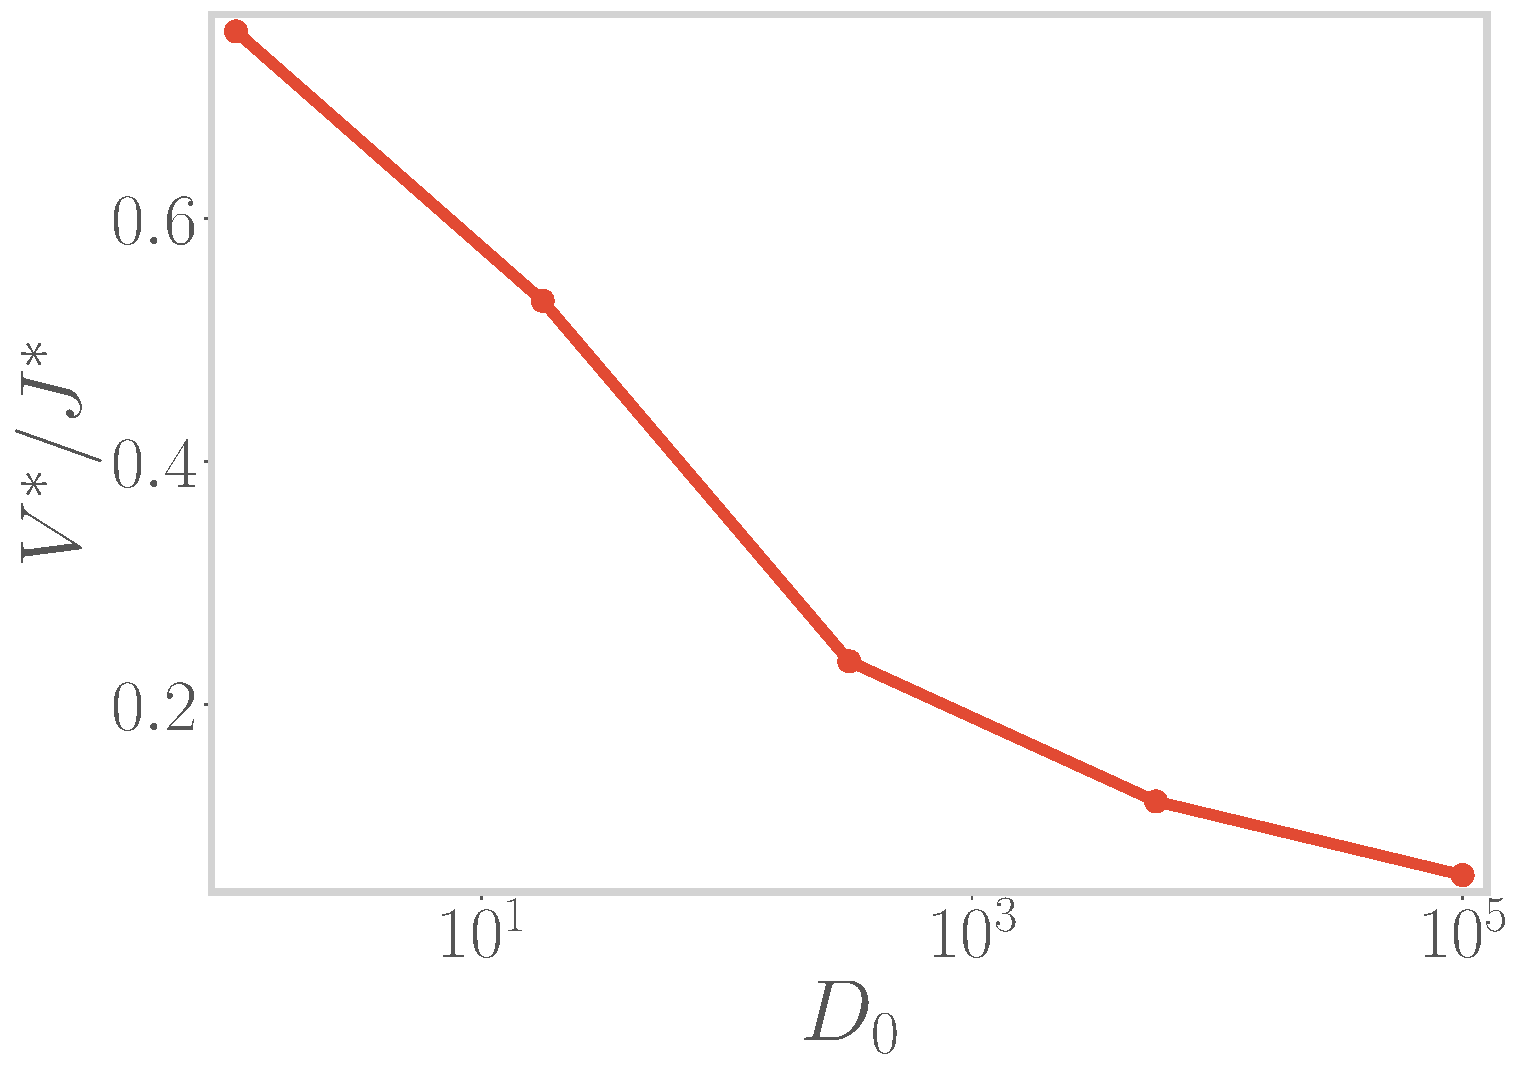
\includegraphics[width=0.48\textwidth]{J_bandwidth.pdf}
	\caption{Increase of \(J^*\) in comparison to \(V^*\) when going towards the thermodynamic limit.}
	\label{J_bandwidth}
\end{figure}

Since the high momentum modes have been decoupled, the ground state in this regime can be estimated by compressing the kinetic energy to the zero bandwidth limit: 
\begin{equation}\begin{aligned}
	\sum_{\sigma,\vec k:|\epsilon_{\vec k}| < D^*} \epsilon_{\vec k} \tau_{\vec k,\sigma} \sim \epsilon_F \sum_{\vec k_F,\sigma}\tau_{\vec k_F,\sigma}
\end{aligned}\end{equation}
Choosing the chemical potential such that \(\epsilon_F\) vanishes results in a {\it two-site Hamiltonian} composed of the impurity site and the zeroth site (see Fig.~\ref{zero-bw}):
\begin{equation}
	\label{two-site}
	H_\text{eff}^\text{sc} \sim J^* \vec{S}_d\cdot\vec{S}_0 - U_b \hat n_{0 \uparrow} \hat n_{0 \downarrow}
\end{equation}
\begin{figure}[!htb]
	\centering
	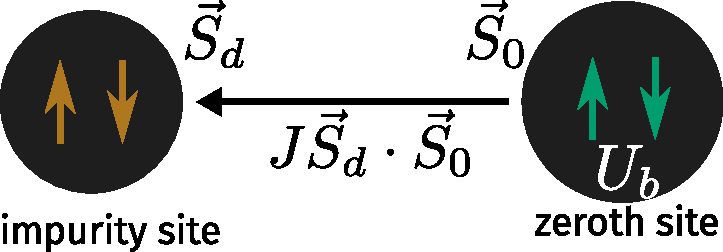
\includegraphics[width=0.4\textwidth]{zeromode_eff.pdf}
	\caption{Two site Hamiltonian obtained by taking the zero bandwidth limit of the effective Hamiltonian in the screened regime.}
	\label{zero-bw}
\end{figure}
This model is easily solved and the ground state is a maximally-entangled spin singlet formed by \(\vec S_d\) and \(\vec S_0\); the ground state energy is \(E_\text{gs}^\text{sc} = -\frac{3}{4}J^* - U_b\):
\begin{equation}\begin{aligned}
	\ket{\Psi}_\text{gs}^\text{sc} = \frac{1}{\sqrt 2}\left(\ket{\uparrow_d,\downarrow_0} - \ket{\downarrow_d,\uparrow_0}\right)
\end{aligned}\end{equation}
where \(\left\{\uparrow_d, \downarrow_d\right\}, \left\{\uparrow_0, \downarrow_0\right\}\) are the spin states of the impurity and zeroth sites respectively. As mentioned before, this regime in the GAIM is adiabatically connected to the AIM, and indeed, such a spin-singlet ground state is also obtained in the AIM from other methods like Poor Man's scaling~\cite{anderson1969exact,anderson1970}, numerical renormalisation group~\cite{wilson1975,hrk_wilson_1980}, the Bethe ansatz~\cite{andrei_1980,andreiKondoreview,Wiegmann_1981,tsvelickKondoreview}, bosonization~\cite{kotliar_1996,Duki_2011,borda_2008}, functional renormalisation group~\cite{streib_2013} and the URG analysis of the Kondo model~\cite{anirban_kondo}.

\subsection{Unscreened regime}

This regime is simpler than the screened regime, because both \(V\) and \(J\) are irrelevant, and only \(U\) is relevant. The effective Hamiltonian then consists of an impurity spin that is decoupled from the conduction bath:
\begin{equation}\begin{aligned}
	H_\text{eff}^\text{uns} = -\frac{1}{2}U^*\left(\hat n_{d \uparrow} - \hat n_{d \downarrow}\right)^2 - U_b \hat n_{0 \uparrow} \hat n_{0 \downarrow} + \sum_{\sigma,\vec k:|\epsilon_{\vec k}| < D^*} \epsilon_{\vec k} \tau_{\vec k,\sigma}
\end{aligned}\end{equation}
The impurity site has a doubly-degenerate ground state \(\left\{ \ket{\uparrow_d}.\ket{\downarrow_d}\right\}\), and the total ground state is the impurity state in direct product with the ground state \(\ket{\Psi}_\text{gs, bath}\) of the conduction bath Hamiltonian \(H_\text{eff, bath}^\text{uns} =  - U_b \hat n_{0 \uparrow} \hat n_{0 \downarrow} + \sum_{\sigma,\vec k:|\epsilon_{\vec k}| < D^*} \epsilon_{\vec k} \tau_{\vec k,\sigma}\):
\begin{equation}\begin{aligned}
	\ket{\Psi}_\text{gs}^\text{uns} = \ket{\sigma_d}\otimes\ket{\Psi}_\text{gs, bath}, ~ ~ ~ \sigma = \uparrow,\downarrow
\end{aligned}\end{equation}



\subsection{The critical point: \(4U_b + J = 0\)}

Along the critical points, \(J\) is marginal and \(U\) is irrelevant, while \(V\) is slightly relevant (see Fig.~\ref{rg-flow}). This leads to enhanced fluctuations in both the spin and charge sectors of the impurity site. The effective Hamiltonian is
\begin{equation}\begin{aligned}
	H_\text{eff}^\text{crit} = \sum_{\sigma,\vec k:|\epsilon_{\vec k}| < D^*} \epsilon_{\vec k} \tau_{\vec k,\sigma} - U_b^* \hat n_{0 \uparrow} \hat n_{0 \downarrow} + J^* \vec{S}_d\cdot\vec{S}_0\\
	+ V^*\sum_\sigma \left( c^\dagger_{d\sigma}c_{0\sigma} + \text{h.c.}\right) 
\end{aligned}\end{equation}

\subsection{Nature of ground state near the critical point}

We can obtain more insight on the change in the ground state as the system moves towards the transition by tracking its overlap with the singlet state \(\ket{\text{ss}} \equiv \ket{\Psi}_\text{gs}^\text{sc}\) and the entangled state among the charge isospin triplets, \(\ket{\text{ct}} \equiv \frac{1}{\sqrt 2}\left(\ket{\uparrow_d \downarrow_d,0} + \ket{0,\uparrow_0 \downarrow_0}\right)\). The ground state \(\ket{\Psi}_\text{gs}\)is obtained by numerically solving the fixed point Hamiltonian for various bare values of the couplings. The overlaps are shown in Fig.~\ref{overlaps}, and we see a continuous increase in the charge content at the cost of the spin content as \(r\) approaches the critical value \(r_c = 0.25\). The spin and charge overlaps approach equality towards the transition, leading to an {\it extra emergent symmetry of spin-charge interchange} at the critical point.

\begin{figure}[!htb]
	\centering
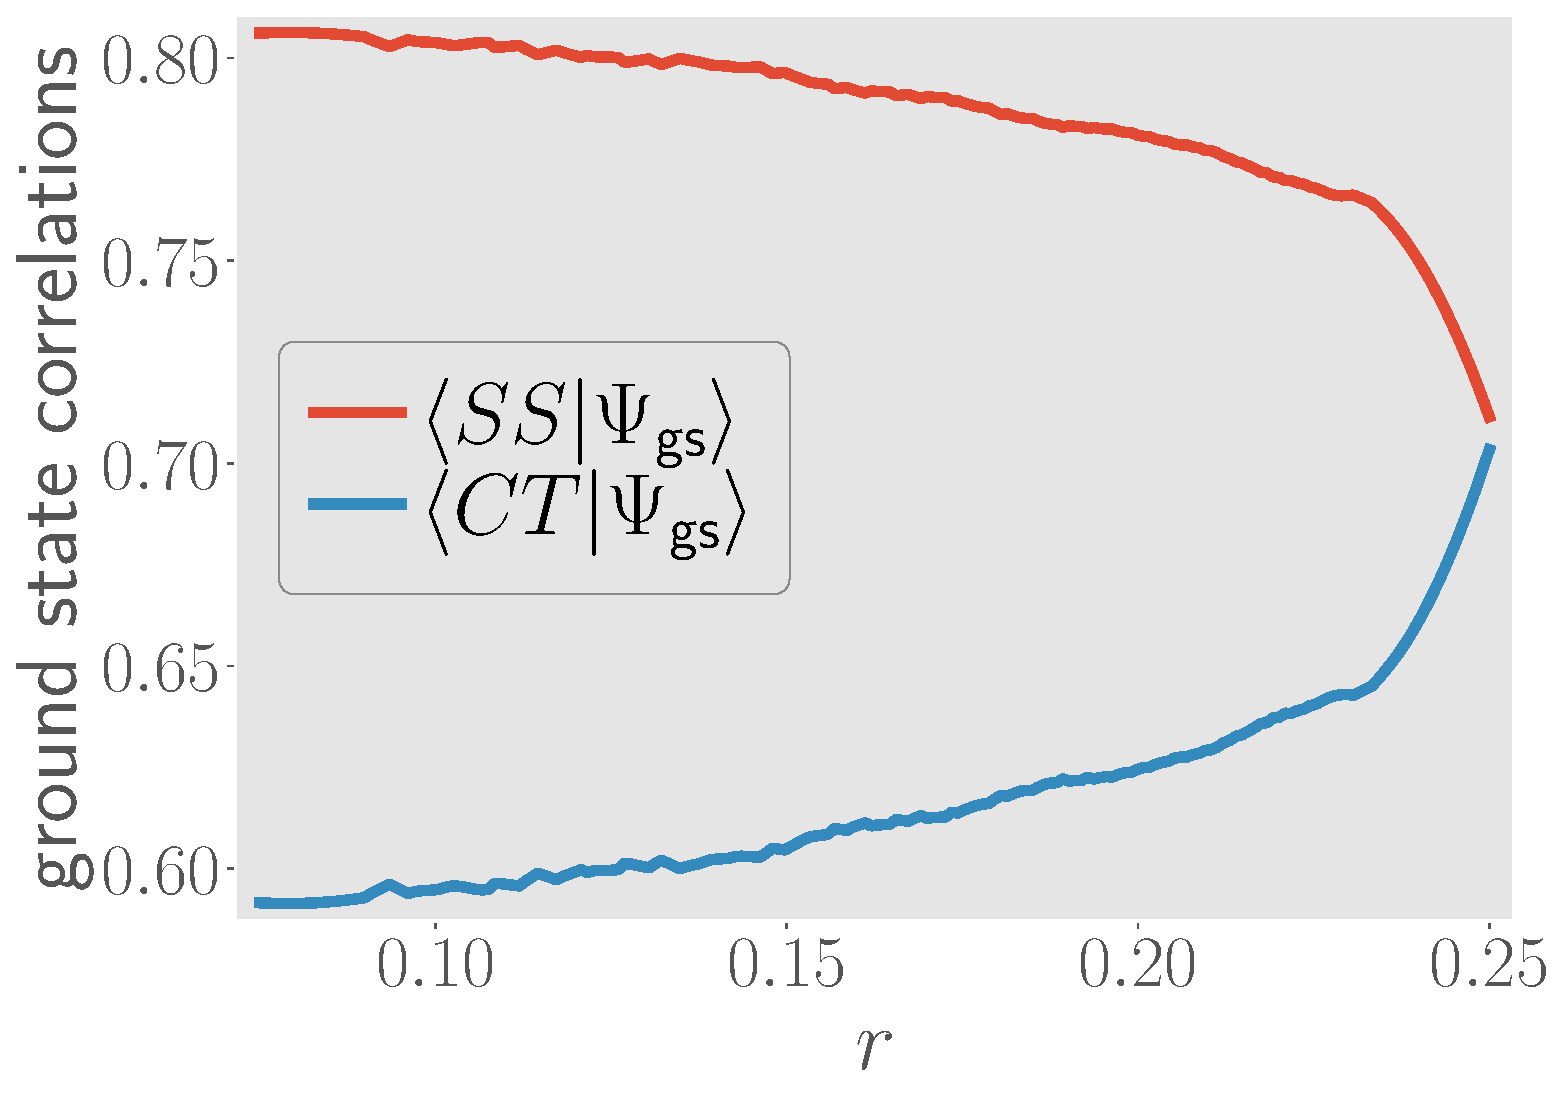
\includegraphics[width=0.48\textwidth]{corrs_gs.pdf}
\caption{Overlap of the RG fixed point ground state \(\ket{\Psi}_\text{gs}\) with the spin singlet state \(\ket{\text{ss}}\) and the charge triplet state \(\ket{\text{ct}}\), for a range of values of the transition tuning ratio \(r\). Beyond the critical point \(r > 0.25\), both these overlaps vanish.}
	\label{overlaps}
\end{figure}


\section{Descriptors of the transition}
\label{descr}

In this section, we will discuss various diagnostics that track the impurity phase transition; these diagnostics or probes will answer several interesting questions:
\begin{itemize}
	\item[1.] How is spectral weight transferred across energy scales, as the system undergoes the transition?
	\item[2.] How do entanglement measures behave across the transition?
	\item[3.] How does the Kondo screening cloud~\cite{sorensen_erik_affleck_1996,affleck_ian_2001,simon_pascal_2003,martin2010,martin2019} respond as the system is driven critical?
\end{itemize}

\subsection{Impurity spectral function}

One of the most obvious indicators of the transition is the appearance of a gap in the spectral function \(A_d(\omega)\) of the impurity. In the AIM, the spectral function \(A_d\) has a single peak structure for small \(U\), and two additional side peaks appear at large \(U\). Although the central peak keeps getting sharper as \(U\) is increased, it never disappears, simply because the impurity is always able to bind with the zeroth site and form a single site; indeed, it is the local Fermi liquid excitations that appear on top of this singlet ground state that gives rise to the central Abrikosov-Suhl resonance in the spectral function~\cite{}[lots of CITE here].

In contrast, the GAIM shows the appearance of a gap as \(r\) crosses \(1/4\) (see Fig.~\ref{spec-func}); the three-peak form survives only up to the critical point. The spectral functions are calculated by numerically diagonalising the effective Hamiltonian obtained from the RG. In the unscreened regime \(r > 0.25\), the impurity spectral function has a two peaks at energies \(\omega = \pm U/2\) corresponding to the fluctuations that create a particle or a hole on the impurity site. The appearance of the gap shows that exactly at \(r=0.25\), the zero-energy pole in the impurity Greens function \(G_d(\omega)\) gets replaced by a zero; this is accompanied by a zero energy divergence in the impurity self-energy \(\Sigma_d = 1/G_d^{(0)}(\omega) - 1/G_d(\omega)\). The expression of the self-energy follows from Dyson's equation, \(G_d^{(0)}(\omega)\) being the self-energy of the impurity at \(U=0\).

\begin{figure}[!htb]
	\centering
	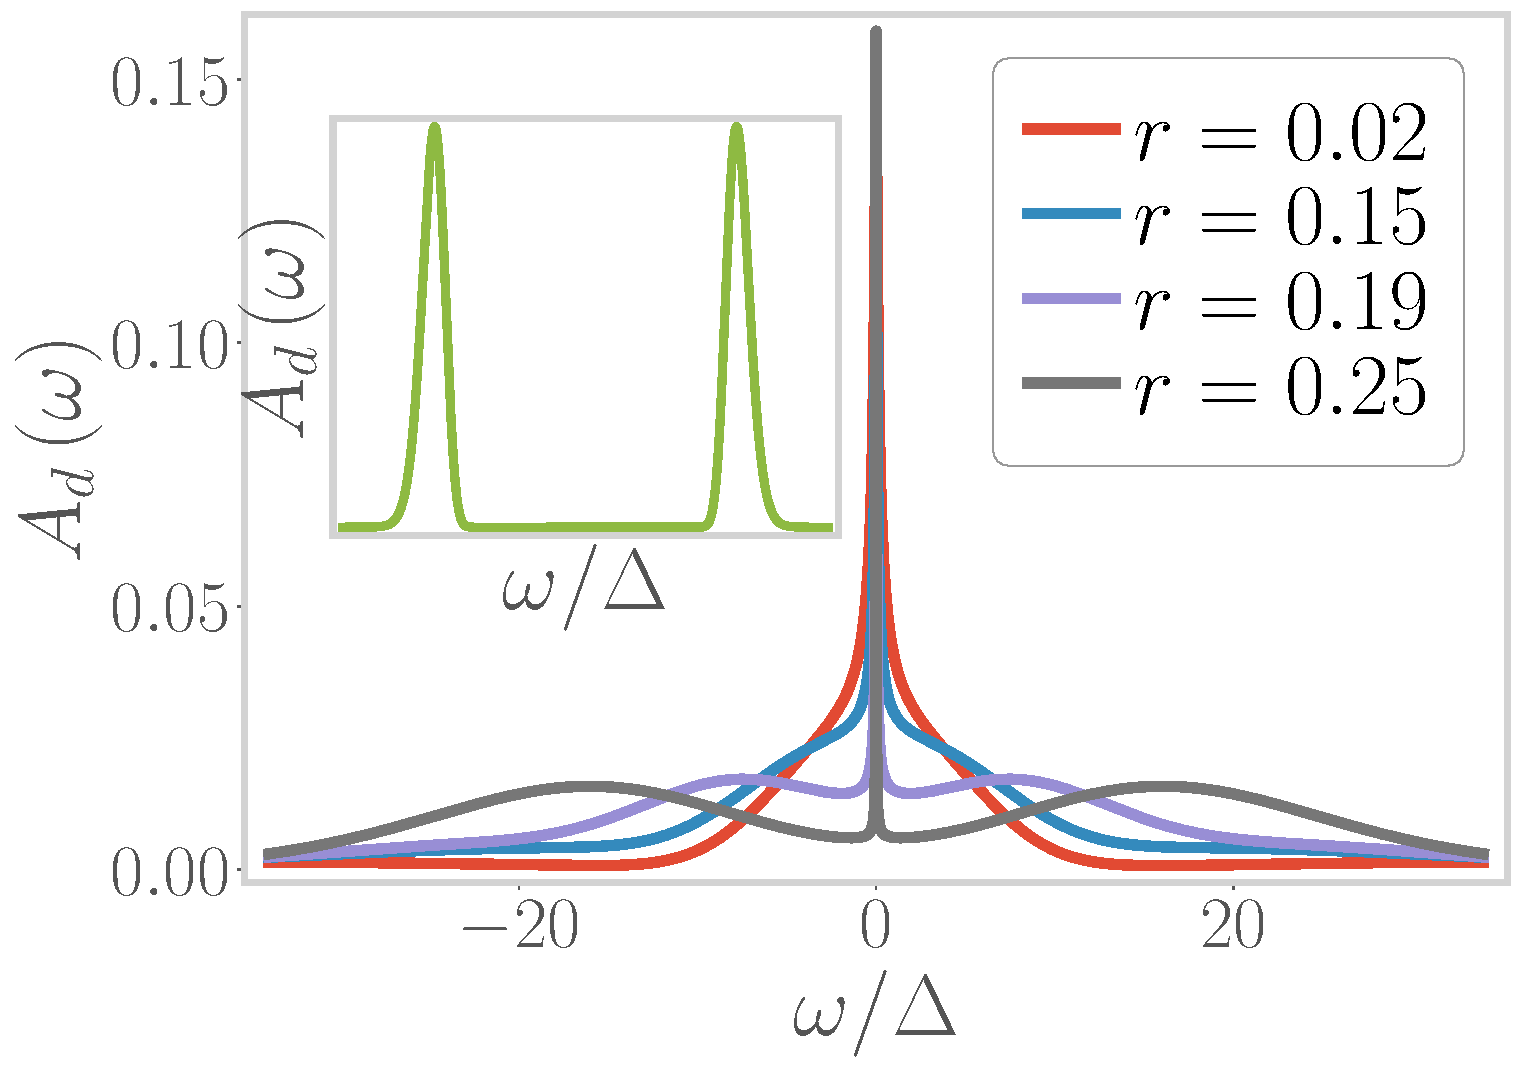
\includegraphics[width=0.48\textwidth]{Add.pdf}
	\caption{Impurity spectral function \(A_d(\omega)\) at three values of the ratio \(r\). The central large plot is exactly at the critical point \(r=0.25\), the left (blue) inset is at \(r < 0.25\) and the right (violet) inset is at \(r > 0.25\).}
	\label{spec-func}
\end{figure}

\subsection{Using geometric entanglement to track the transition}

Given a ground state \(\ket{\Psi}_\text{gs}\) and a spectrum of energies \(\left\{ E_n \right\} \), the impurity Greens function can be given a spectral representation in terms of the eigenstates \(\left\{\ket{\Psi}_n\right\}\) of the GAIM:
\begin{equation}\begin{aligned}
G_d(\omega) = \sum_n \left[ \frac{|\braket{\Psi_\text{gs} | c_{d\sigma} | \Psi_n}|^2}{\omega + E_\text{gs} - E_n} + \frac{|\braket{\Psi_n | c_{d\sigma} | \Psi_\text{gs}}|^2}{\omega - E_\text{gs} + E_n}\right] 
\end{aligned}\end{equation}
We will now introduce a complete basis into the expression. The basis will be the set of eigenstates of the Hamiltonian  \(H = H_1 + H_2\), where \(H_1\) is the two-site Hamiltonian in eq.~\ref{two-site}, and \(H_2\) is a tight-binding Hamiltonian formed by the remaining sites. Since the Hamiltonians are decoupled, the eigenstates \(\ket{\Psi}_{m,n}\) will be direct product states formed by combining the eigenstates \(\ket{\phi}_m,\ket{\psi}_n\) of the individual Hamiltonians \(H_1\) and \(H_2\) respectively: \(\ket{\Phi}_{m,n} = \ket{\phi}_m\otimes\ket{\psi}_n\). Inserting this basis leads to the expression:
\begin{equation}\begin{aligned}
	\label{summation}
	\ket{\Psi}_\text{gs} = \sum_{m,n} \ket{\Phi}_{m,n} \left(\bra{\phi_{m}}\otimes\bra{\psi_n}\right)\ket{\Psi_\text{gs}}
\end{aligned}\end{equation}
The ground state of \(H_1\) is the spin singlet: \(\ket{\phi}_0 = \ket{\text{ss}}\). We denote the ground state of the tight-binding Hamiltonian \(H_2\) by \(\ket{\psi}_0\). Because of the highly renormalised couplings \(V\) and \(J\), the impurity site is almost maximally entangled with the zeroth site, such that the ground state \(\ket{\Psi}_\text{gs}\) in the \(r < 0.25\) regime can be thought of as a direct product of the two-site ground state, \(c\ket{\text{ss}} + \sqrt{1-c^2}\ket{\text{ct}}\), in direct product with the tight-binding ground state:
\begin{equation}\begin{aligned}
	\ket{\Psi}_\text{gs} \simeq \left(c\ket{\text{ss}} + \sqrt{1-c^2}\ket{\text{ct}}\right)  \otimes \ket{\psi}_0 = \ket{\Phi}_\text{ss} + \ket{\Phi}_\text{ct}
\end{aligned}\end{equation}
where \(\ket{\Phi}_\text{ss(ct)} = \ket{\text{ss}\left( \text{ct} \right)}\otimes\ket{\psi}_0 \).
This suggests that not all terms in the summation of eq.~\ref{summation} contribute; out of all \(\left\{ \ket{\psi}_n \right\} \), only the ground state \(n=0\) contributes, while only \(\ket{ss}\) and \(\ket{ct}\) contribute from the set \(\left\{ \ket{\phi}_m \right\} \). The summation then simplifies to
\begin{equation}\begin{aligned}
	\ket{\Psi}_\text{gs} = \ket{\Phi}_{ss}\braket{\text{ss}|\Psi^{(2)}_\text{gs}} + \ket{\Phi}_{ct}\braket{\text{ct}|\Psi^{(2)}_\text{gs}}~,
\end{aligned}\end{equation}
where \(\ket{\Psi^{(2)}_\text{gs}}\) is the two-site part of the ground state and can be obtained by starting with the full ground state \(\ket{\Psi}_\text{gs}\) and tracing over the other lattice sites of the system.

We assume that the global phase of the wavefunctions are real, and since the internal weights of the wavefunctions are real as well, the overlaps \(\braket{\text{ss}|\Psi^{(2)}_\text{gs}},\braket{\text{ct}|\Psi^{(2)}_\text{gs}}\) are also real. We can use these overlaps to define a geometric measure of entanglement~\cite{shimony1995degree,wei2003geometric,horodecki2009quantum}:
\begin{equation}\begin{aligned}
	\varepsilon\left(\psi_1,\psi_2\right) = 1 - |\braket{\psi_1 | \psi_2}|^2
\end{aligned}\end{equation}
If \(\ket{\psi_1}\) is thought of as a separable state, then \(\ket{\psi_2}\) should be less entangled if it's overlap with \(\ket{\psi_1}\) is large, which is indeed borne out by the definition.
The overlaps then become \(\braket{\text{ss}|\Psi^{(2)}_\text{gs}} = \sqrt{1 - \varepsilon\left(ss,\Psi^{(2)}_\text{gs}\right)}\), and similarly for the state \(\ket{\text{ct}}\). For brevity, we will use the notation \(\varepsilon_\text{ss} \equiv \varepsilon\left(ss,\Psi^{(2)}_\text{gs}\right), \varepsilon_\text{ct} \equiv \varepsilon\left(ct,\Psi^{(2)}_\text{gs}\right)\). The Greens function can now be written in terms of these measures:
\begin{widetext}
\begin{equation}\begin{aligned}
	G_d(\omega) = \sum_n \left[\left(1 - \varepsilon_\text{ss} \right) \left(\frac{|\braket{\Phi_\text{ss} | c_{d\sigma} | \Psi_n}|^2}{\omega + E_\text{gs} - E_n} + \frac{|\braket{\Psi_n | c_{d\sigma} | \Phi_\text{ss}}|^2}{\omega - E_\text{gs} + E_n}\right) + \left(1 - \varepsilon_\text{ct} \right) \left(\frac{|\braket{\Phi_\text{ct} | c_{d\sigma} | \Psi_n}|^2}{\omega + E_\text{gs} - E_n} + \frac{|\braket{\Psi_n | c_{d\sigma} | \Phi_\text{ct}}|^2}{\omega - E_\text{gs} + E_n}\right)\right.\\
	+ \left. \sqrt{\left(1 - \varepsilon_\text{ss} \right)}\sqrt{\left(1 - \varepsilon_\text{ct} \right)} \left(\frac{\braket{\Phi_\text{ss} | c_{d\sigma} | \Psi_n}\braket{\Psi_n | c^\dagger_{d\sigma} | \Phi_\text{ct}} + \text{h.c.}}{\omega + E_\text{gs} - E_n} + \frac{\braket{\Phi_\text{ct} | c_{d\sigma} | \Psi_n}\braket{\Psi_n | c^\dagger_{d\sigma} | \Phi_\text{ss}} + \text{h.c.}}{\omega - E_\text{gs} + E_n}\right)\right]
\end{aligned}\end{equation}
\end{widetext}

\begin{figure}[!htb]
	\centering
	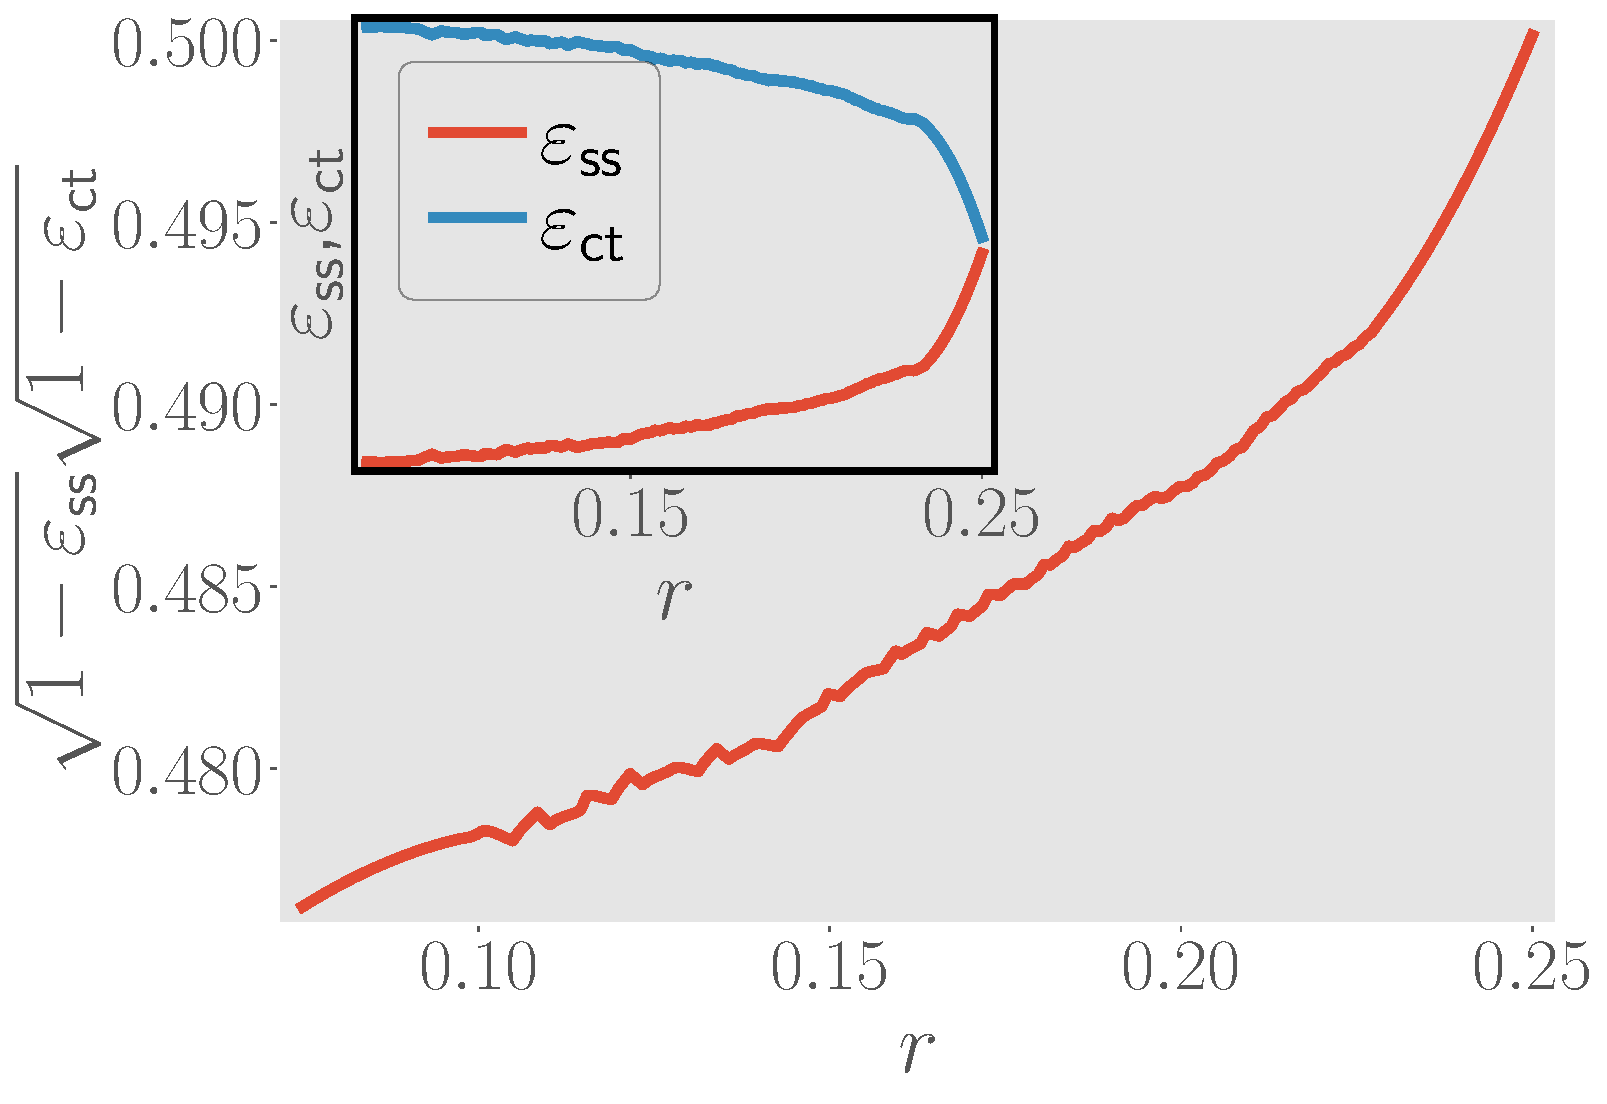
\includegraphics[width=0.48\textwidth]{entanglement.pdf}
	\caption{Variation of \(\sqrt{\left(1 - \varepsilon_\text{ss} \right)}\sqrt{\left(1 - \varepsilon_\text{ct} \right)}\) as \(r\) is increased towards the critical value 0.25. Inset shows the variation of the individual measures \(\varepsilon_\text{ss},\varepsilon_\text{ct}\).}
	\label{entng}
\end{figure}

This expression is interesting because it relates the Greens function (measurable when converted into a spectral function) to measures of entanglement.
These measures have been plotted up to the critical point in Fig.~\ref{entng}.
While \(\varepsilon_\text{ss},\varepsilon_\text{ct}\) (plotted in the inset) are very similar to the overlaps plotted in Fig.~\ref{overlaps}, the cross-term \(\sqrt{\left(1 - \varepsilon_\text{ss} \right)}\sqrt{\left(1 - \varepsilon_\text{ct} \right)}\) plotted in the main figure has an overall monotonic incremental behaviour towards the transition.
We can now use the knowledge of the behaviour of these measures to make some statements about the nature of the transition from the Greens function.
Since \(\varepsilon_\text{ss}\) increases towards the transition, we find that the first major term in the Greens function decreases; this shows that scattering within the spin sector loses weight.
On the other hand, since \(\varepsilon_\text{ct}\) decreases, the second major term in \(G_d\) increases, reflecting the growth in the participation of the charge sector in the scattering processes.
The final major term also increases, due to the monotonic growth of \(\sqrt{\left(1 - \varepsilon_\text{ss} \right)}\sqrt{\left(1 - \varepsilon_\text{ct} \right)}\), showing that there is a continual increase in the {\it mixing of the spin and charge sectors}.

\subsection{Mutual information and spin/charge correlations in ground state: fate of the Kondo cloud}
Since the system has to undergo a phase transition into an unscreened phase for \(r > 0.25\), it is clear that the Kondo screening cloud must disappear. Indeed, this is captured by various entanglement measures like mutual information and entanglement entropy. The entanglement entropy (EE) \(S(A)\) of subsystem \(A\) with the rest of the system is defined as the von Neumann entropy of the reduced density matrix \(\rho_A\),
\begin{equation}\begin{aligned}
	S(A) = -\text{Tr}\left[\rho_A \ln \rho_A\right]~,
\end{aligned}\end{equation}
where \(\rho_A\) is obtained by tracing the full density matrix \(\rho = \ket{\Psi}_\text{gs} \bra{\Psi}_\text{gs}\) over all subsystems apart from \(A\). The mutual information between two subsystems \(A\) and \(B\) is then defined using this entanglement entropy:
\begin{equation}\begin{aligned}
	I(A:B) = S(A) + S(B) - S(A \cup B)~,
\end{aligned}\end{equation}
where \(S(A \cup B)\) is the EE of \(A\) and \(B\) with the rest. \(I(A:B)\) represents the amount of information obtained about \(B\) on measuring \(A\), or vice-versa. If the ground state \(\ket{\Psi}_\text{gs}\) is a state that is separable in terms of \(A\) and \(B\), then the system can be split into two disjoint parts, one of which is coupled to A and the other coupled to B.  The total EE from both \(A\) and \(B\) is then just a sum of its parts: \(S(A\cup B) = S(A) + S(B)\), such that \(I(A:B) = 0\). On the other hand, if the ground state cannot be written in separable form, the EE of the sum, \(S(A \cup B)\) is more than the sum of its parts because of the additional entanglement between \(A\) and \(B\), and we get \(I(A:B) > 0\). In recent times, such measures of entanglement have often been used to study Kondo impurity~\cite{Srensen2006}, heavy-fermionic~\cite{parisen_2019} and other impurity systems~\cite{dong_2021}.

\begin{figure}[!htb]
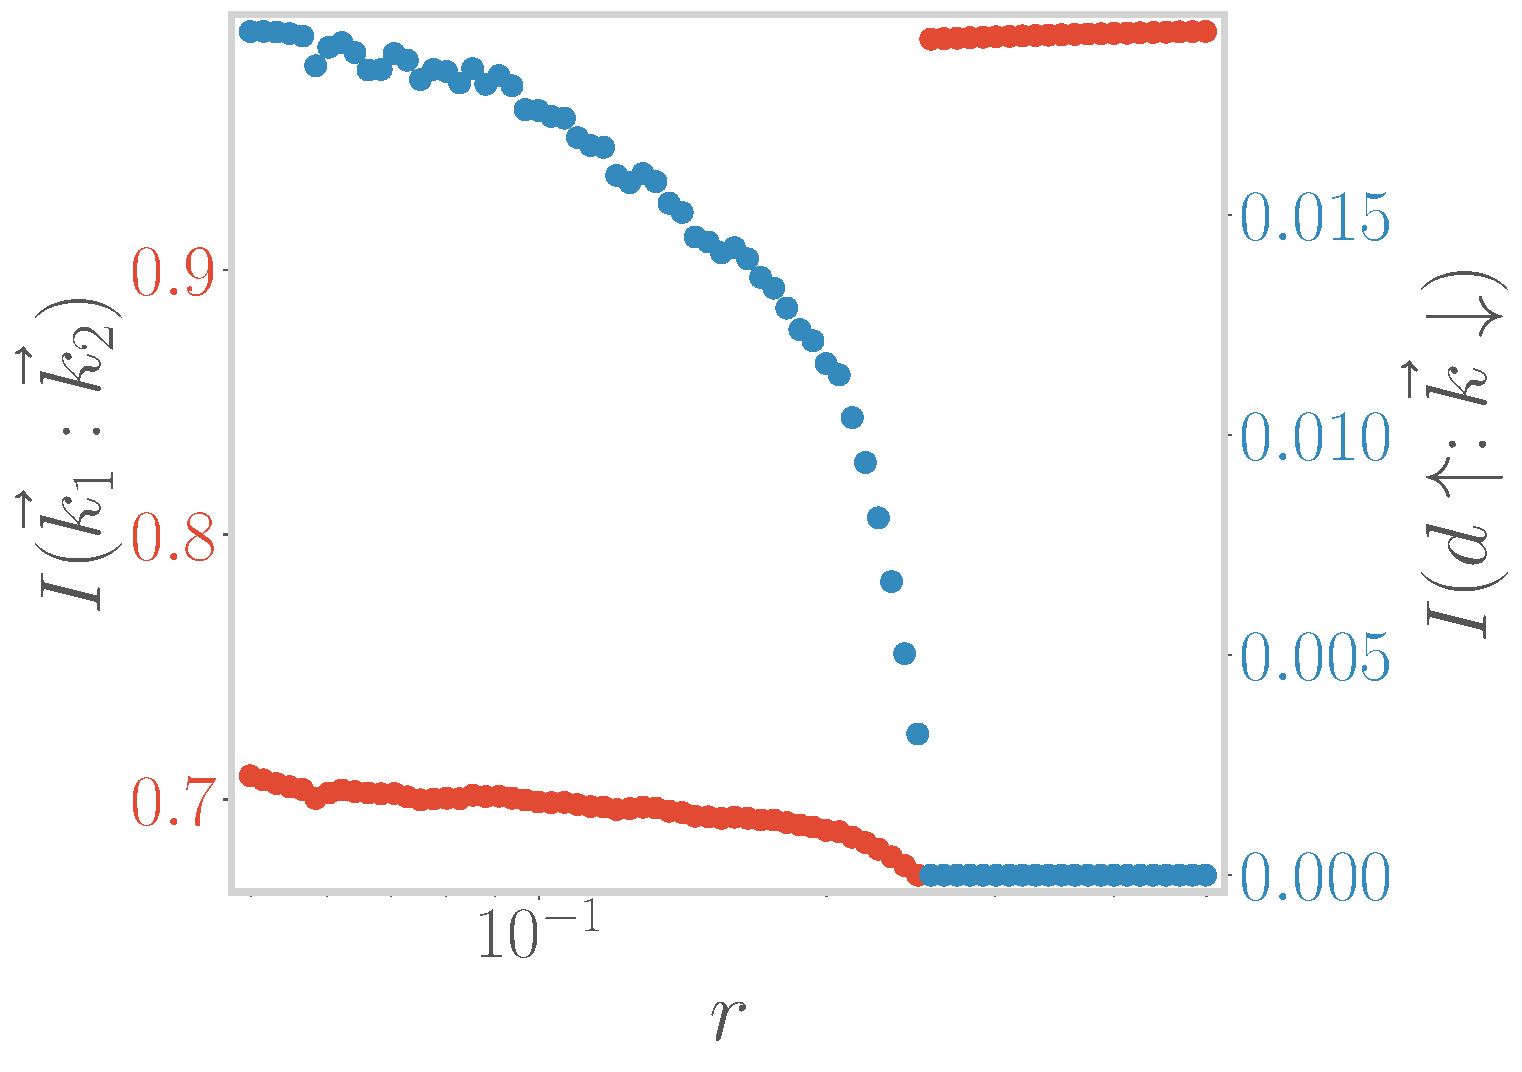
\includegraphics[width=0.49\textwidth]{I_k.pdf}
\caption{Mutual information in \(k-\)space, across the transition. Red curve is the mutual information between two distinct \(k-\) states inside the Kondo cloud. Blue curve is the mutual information between a \(k-\)state and the impurity state of opposite spin.}
\label{mut_inf_k}
\end{figure}

In the AIM or the Kondo model ground state, the impurity forms a maximally entangled singlet with the zeroth site~\cite{wilson1975,hewson1993,hrk_wilson_1980}.
This in turn leads to entanglement in \(k-\)space between the conduction electrons that screen the impurity and form the Kondo cloud~\cite{anirban_kondo}.
These features change once we turn on the attractive correlation \(U_b\) and drive the system across the transition, as plotted in Figs.~\ref{mut_inf_k} and \ref{mut_inf_r}.
The \(k-\)space mutual information \(I(\vec k_1:\vec k_2)\) between two distinct \(k-\)states plotted in the red curve of Fig.~\ref{mut_inf_k} is essentially the entanglement within the Kondo cloud, and we find that this entanglement decreases towards the transition, signalling the weakening of the Kondo cloud.
This is also supported by the reduction in the mutual information \(I(d \uparrow: \vec k \downarrow)\) between the impurity and \(k-\)space states plotted along the blue curve in the same figure. Beyond the transition, \(I(d \uparrow: \vec k \downarrow)\) drops to zero, because the impurity is no longer coupled to the bath, while \(I(\vec k_1:\vec k_2)\) takes on a larger value because they are connected by the \(U_b-\)term and are no longer sharing entanglement with the impurity.

\begin{figure}[!htb]
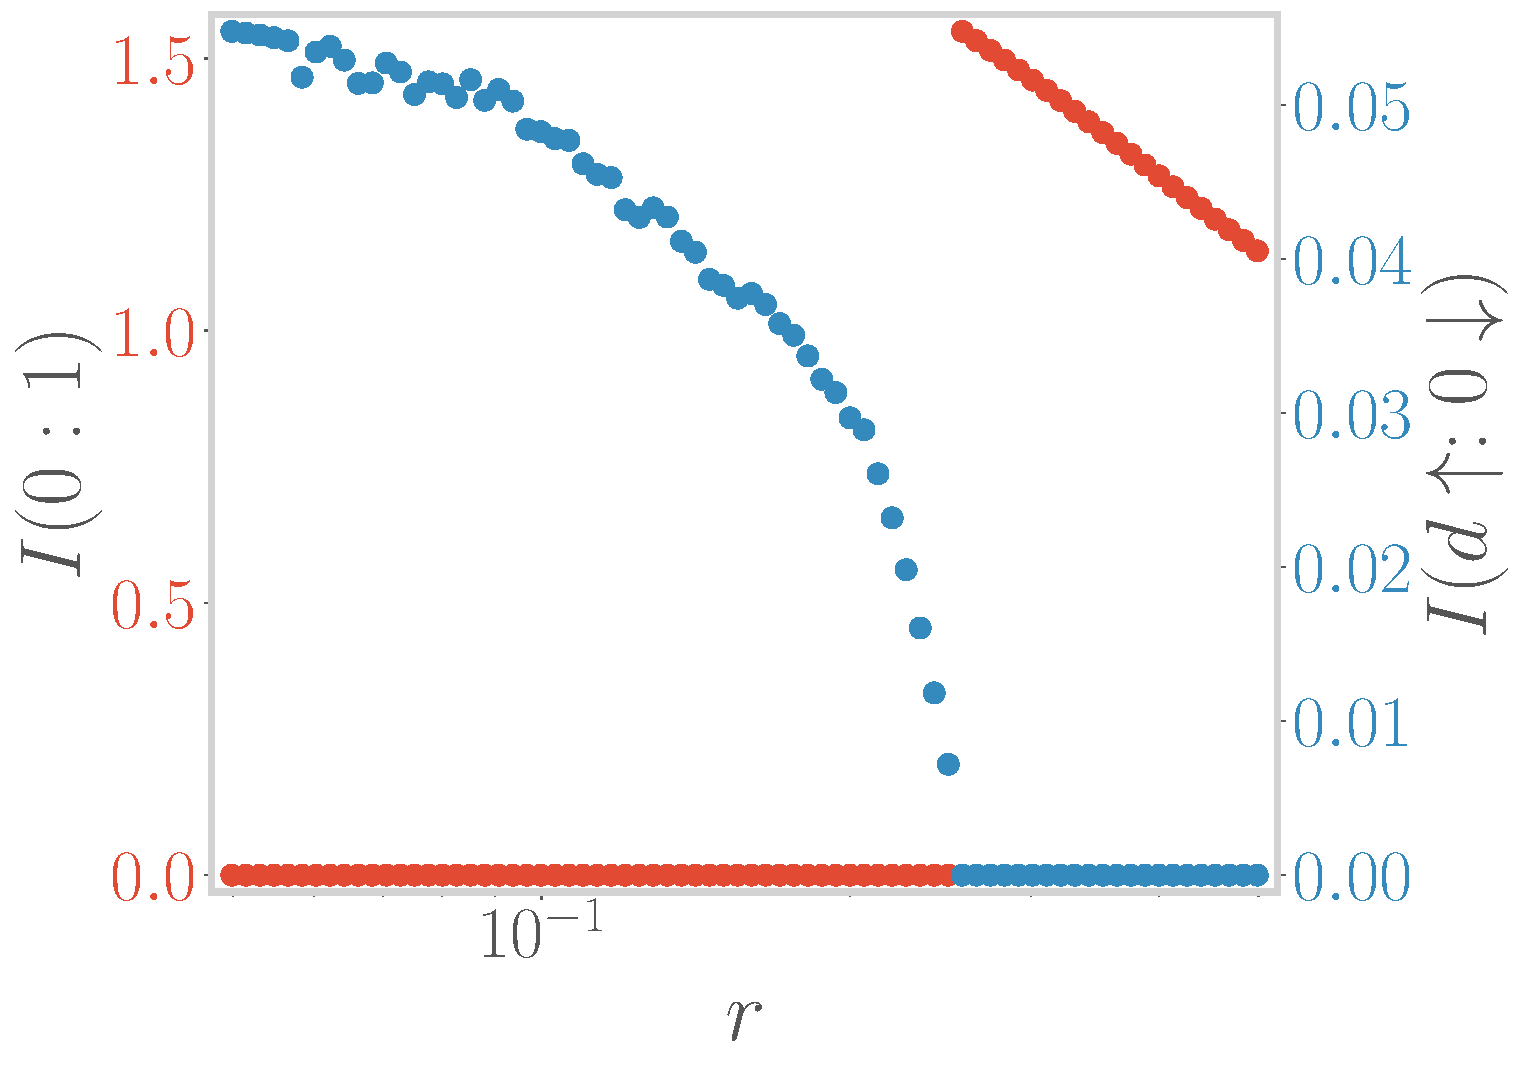
\includegraphics[width=0.49\textwidth]{I_r.pdf}
\caption{Mutual information in \(r-\)space, across the transition. Red curve is the mutual information between the zeroth site and the site next to it. Blue curve is the mutual information between a \(k-\)state and the impurity state of opposite spin. The former is zero before the transition because the zeroth site is locked in a singlet with the impurity, and becomes zero after  the transition because the singlet has now decoupled and the zeroth site is free to entangle with the other sites.}
\label{mut_inf_r}
\end{figure}

{\color{blue}Apart from the mutual information, we also computed two complimentary measures of correlation in the ground state, the spin-flip and the charge isospin correlations, \(\left<S_d^+ S_0^- \right>\) and \(\left<c^\dagger_{ 0 \uparrow} c^\dagger_{0 \downarrow} c_{d \downarrow} c_{d \uparrow} \right>\) respectively. These are shown in Fig.~\ref{charge-spin}, and show opposite tendencies. While the spin-flips decrease due to the destruction of the Kondo cloud, the charge isospin fluctuations grow because of the attractive correlation \(U_b\). Both drop to zero abruptly beyond the transition, because the impurity entirely decouples from the bath.}

\begin{figure}[!htb]
	\centering
	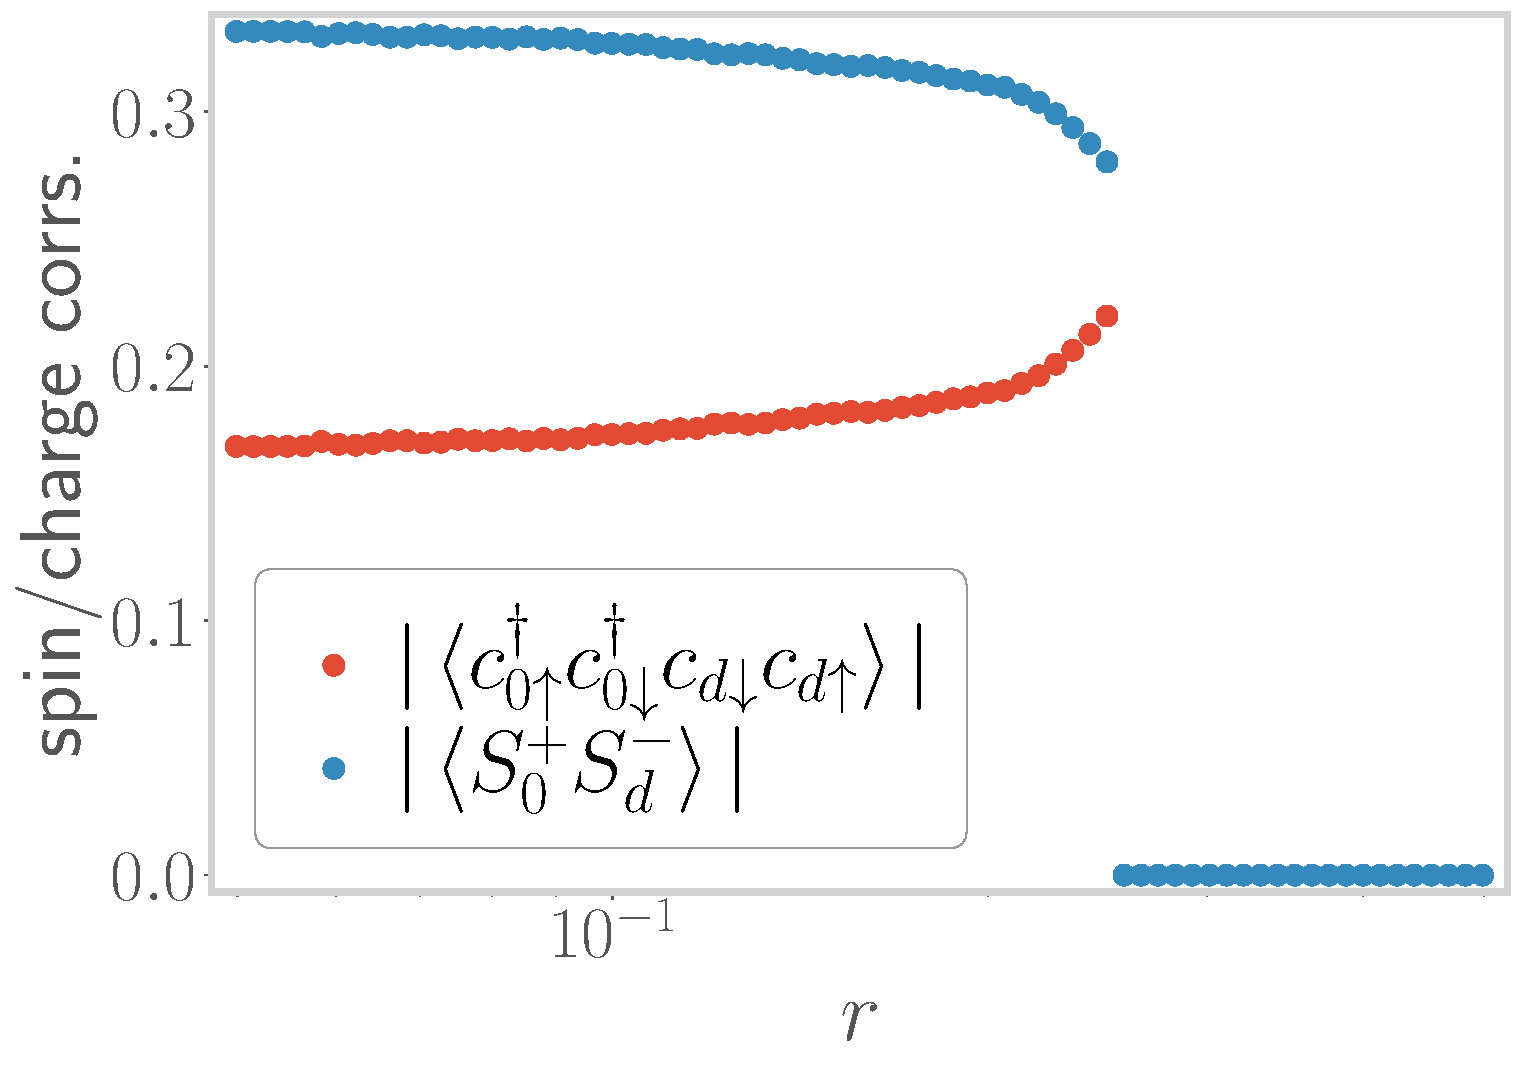
\includegraphics[width=0.48\textwidth]{odlro_d0.pdf}
	\caption{Variation of spin-flip correlation and charge isospin-flip correlation across the transition.}
	\label{charge-spin}
\end{figure}

\section{Discussions and Outlook}
\label{concl}

In summary, we have shown that adding spin-exchange physics between impurity and bath and local atractive correlation in the bath lead to a model with multiple phases. We have demonstrated this phase transition under a renormalisation group treatment, and provided the effective Hamiltonians and simplified wavefunctions for the various phases. The phase transition can be observed through the discontinuous behaviour in the ground state, as well as through the appearance of a gap in the impurity spectral function. We also draw a connection between the change in the spectral function and some geometric measures of entanglement; this allows tracking the phase transition via these measures.

Having summarised the main results, we now discuss some additional notable insights. We note that the GAIM as defined here represents the most minimal impurity model that supports a phase transition - both the \(J\) and \(U_b\) are crucial to stabilising the local moment. With just \(J\) or just \(U_b\), the low-energy phase is always of the local Fermi liquid kind. The introduction of the attractive \(U_b\) term is most interesting because it shows that pairing fluctuations in the bath are necessary to suppress the Kondo physics arising from spin fluctuations(fig.~\ref{pair_fluc}). Moreover, we find that there is a subdominant tendency towards transfer of local ``Cooper pairs" between the impurity and zeroth sites (Fig.~\ref{charge-spin}). This is reminiscent of a similar subdominant superconducting tendency in the half-filled Hubbard model as observed from a unitary RG treatment~\cite{anirbanmott1,anirbanmott2}.
It is also intriguing to see that the geometric entanglement \(\chi = \sqrt{1 -\varepsilon_\text{SS}}\sqrt{1 -\varepsilon_\text{CT}}\) emerges as an order parameter for the impurity transition: it is zero in the local moment phase and non-zero in the screened phase. The discontinuous change in \(\chi\) is intimately connected to the fact that this phase transition is topological in nature~\cite{oshikawa2000topological,seki2017topological} -  the Luttinger volume of the conduction bath changes by 1~\cite{martin-physrevlett.48.362}.

Future studies can involve working with a general filling on the impurity site; this might allow the pair fluctuations between the impurity and zeroth site to become the dominant interaction, leading to a "local superconducting instability".
Another important application of this model involves the following: Given a suitable analytical framework, the auxiliary model obtained here can be ``tiled" throughout the lattice to create a bulk model, and the impurity phase transition observed here will then get promoted to a bulk metal-insulator transition.
Finer details like electronic differentiation in \(k-\)space can also be captured by taking more number of impurities in the auxiliary model~\cite{sakai_2009}.


\acknowledgments
Abhirup Mukherjee thanks IISER Kolkata for funding through a research fellowship. S. Lal thanks the SERB, Govt. of India for funding through MATRICS grant MTR/2021/000141 and Core Research Grant CRG/2021/000852.

\bibliography{gen-siam}

\appendix*

\section{Derivation of RG equations for the generalised Anderson impurity model}

\subsection{Some preliminaries}
The Hamiltonian we are working with is the generalised Anderson impurity model (Eq.~\ref{GIAM-ham}):
\begin{equation}\begin{aligned}
	\mathcal{H} = -\frac{1}{2}U \left(\hat n_{d \uparrow} - \hat n_{d \downarrow}\right)^2 + \sum_{\vec k,\sigma} \epsilon_{\vec k} \tau_{\vec k,\sigma} + J \vec{S}_d\cdot\vec{S}_0 \\
	+ V\sum_\sigma \left( c^\dagger_{d\sigma}c_{0\sigma} + \text{h.c.}\right) - U_b \hat n_{0 \uparrow} \hat n_{0 \downarrow}
\end{aligned}\end{equation}
The renormalisation in the Hamiltonian \(H_{(j)}\) at the \(j^\text{th}\) RG step, upon decoupling an electronic state \(q\beta\), is given by the expression:
\begin{equation}\begin{aligned}
	&\left(\Delta H_{(j)}\right)_{\vec q,\beta} = H_{(j-1)} - H_{(j)} \\
	&= c^\dagger_{\vec q,\beta} T_{\vec q,\beta} \frac{1}{\omega_e - H_D} T^\dagger_{\vec q,\beta}c_{\vec q,\beta} + T^\dagger_{\vec q,\beta} c_{\vec q,\beta} \frac{1}{\omega_h - H_D} c^\dagger_{\vec q,\beta}T_{\vec q,\beta}~,
\end{aligned}\end{equation}
where \(\omega_{e,h}\) are the quantum fluctuation scales for the electron and hole scattering channels, \(H_D\) is the part of the Hamiltonian that is diagonal in \(k-\)space, and \(T_{\vec q,\beta} + T_{\vec q,\beta}^\dagger\) is the part of the Hamiltonian that does not commute with \(\hat n_{\vec q,\beta}\) (in short, it is the part that is off-diagonal with respect to a particular state \(\vec q,\beta\)). This off-diagonal part is made up of contributions from \(V,J\) and \(U_b\): \(T_{\vec q \uparrow} = \left[V c^\dagger_{d \uparrow}  + J \sum_{\vec k}S_d^+ c^\dagger_{\vec k \downarrow}  + U_b \sum_{\vec k_1,\vec k_2,\vec k_3}c^\dagger_{\vec k_1 \uparrow} c^\dagger_{\vec k_3 \downarrow} c_{\vec k_4 \downarrow}\right] c_{\vec q \uparrow}\),
while the diagonal part is given by \(H_D = \epsilon_{\vec q} \tau_{q\uparrow} + \frac{1}{4}J S_d^z\left(\hat n_{q \uparrow} - \hat n_{q \downarrow}\right) - U_b \left(\tau_{\vec q,\uparrow}\right)^2\),
where we have rewritten \(\hat n_{\vec q,\beta}\) in terms of \(\tau_{\vec q,\beta} \equiv \hat n_{\vec q,\beta} - \frac{1}{2}\) in the contribution from \(U_b\).

Note that we have ignored a potential scattering term in the off-diagonal part \(T_{\vec q\beta}\). Because the diagonal contribution from \(U_b\) always changes the energy of the excited energy by \(-U_b/4\),  the denominator will simply change by \(U_b/4\) (\(H_D\) comes with a minus sign in the denominator). We will suppress this change for now and substitute in all the denominators at the end. We define \(n_j\) as the number of states being decoupled on each side of the Fermi surface, at the \(j^\text{th}\) RG step. In order to treat both spin and isospin exchanges democratically, we take \(\ket{\Psi}_i = \frac{1}{2}\left(\ket{0} + \ket{q\uparrow} + \ket{q\downarrow} + \ket{q\uparrow, q\downarrow}\right) \) as the \textit{initial} state for the scattering processes. The kinetic energy for \(\ket{\Psi}_\text{int}\) is \(\epsilon_q \tau_{q \uparrow} = \left(-D\right)\times\left(-\frac{1}{2}\right) = D/2\).


\subsection{Renormalisation of \(U_b\)}
\(U_b\) can renormalise only via itself. The relevant renormalisation term in the particle sector is
\begin{equation}\begin{aligned}
	U_b^2 \sum_{q\beta}\sum_{k_1,k_2,k_3,\atop{k_1^\prime,k_2^\prime,k_3^\prime}} c^\dagger_{q\beta}c_{k_1\beta}c^\dagger_{k_3\overline\beta}c_{k_1^\prime\overline\beta}\frac{1}{\omega - H_D}c^\dagger_{k_2^\prime\overline\beta}c_{k_3^\prime\overline\beta}c^\dagger_{k_2\beta}c_{q\beta}
\end{aligned}\end{equation}
In order to renormalise \(U_b\), we need to contract one more pair of momenta. There are two choices. The first is by setting \(k_3 = k_3^\prime = q\). The two internal states, then, are \(q\beta\) and \(q\overline\beta\). As discussed above, the intermediate state energy is \(-U_b/4\). We therefore have
\begin{equation}\begin{aligned}
	\frac{U_b^2 n_j}{\omega - D/2 + \frac{U_b}{2}}\sum_{\beta}\sum_{k_1,k_2,k_1^\prime,k_2^\prime} c_{k_1\beta}c_{k_1^\prime\overline\beta}c^\dagger_{k_2^\prime\overline\beta}c^\dagger_{k_2\beta} \\
	= \frac{U_b^2 n_j}{\omega - D/2 + \frac{U_b}{2}}\sum_{\beta}\sum_{k_1,k_2,k_1^\prime,k_2^\prime} c^\dagger_{k_2^\prime\overline\beta}c_{k_1^\prime\overline\beta}c^\dagger_{k_2\beta}c_{k_1\beta}
\end{aligned}\end{equation}
Another way to contract the momenta is by setting \(k_1^\prime = k_2^\prime = q\), which gives a renormalisation of
\begin{equation}\begin{aligned}
	\frac{U_b^2 n_j}{\omega - D/2 + \frac{U_b}{2}}\sum_{\beta}\sum_{k_1,k_2,k_3,k_3^\prime} c_{k_1\beta}c^\dagger_{k_3 \overline\beta}c_{k_3\prime\overline\beta}c^\dagger_{k_2\beta} \\
	= -\frac{U_b^2 n_j}{\omega - D/2}\sum_{\beta}\sum_{k_1,k_2,k_3,k_3^\prime} c^\dagger_{k_3 \overline\beta}c_{k_3\prime\overline\beta}c^\dagger_{k_2\beta}c_{k_1\beta}
\end{aligned}\end{equation}
The two contributions cancel each other. The same cancellation happens in the hole sector as well.



\subsection{Renormalisation of the impurity correlation \(U\)}
The coupling \(U\) is renormalised by two kinds of vertices: \(V^2\) and \(J^2\). We will consider these processes one at a time. For convenience, we define \(\epsilon_d = -U/2\).

The renormalisation arising from the first kind of terms, in the particle sector, is
\begin{equation}\begin{aligned}
	&\sum_{q\beta}c^\dagger_{q\beta}c_{d\beta}\frac{V^2}{\omega - H_D}c^\dagger_{d\beta}c_{q\beta}\\
	&= \sum_{q\beta}V^2 \hat n_{q\beta} \left( 1 - \hat n_{d\beta} \right)\left( \frac{1-\hat n_{d \overline\beta }}{\omega - E_0} + \frac{\hat n_{d \overline\beta}}{\omega^\prime - E_1}\right) \\
	&= V^2 n_j\sum_{\beta}\left( 1 - \hat n_{d\beta} \right)\left( \frac{1-\hat n_{d \overline\beta }}{\omega_0 - E_0} + \frac{\hat n_{d \overline\beta}}{\omega_1 - E_1}\right)
\end{aligned}\end{equation}
\(q\) runs over the momentum states that are being decoupled at this RG step: \(|q| = \Lambda_j\). \(E_{1,0}\) are the diagonal parts of the Hamiltonian at \(\hat n_{d\overline \beta}=1,0\) respectively: \(E_1 = \frac{D}{2}\) and \(E_0 = \frac{D}{2} + \epsilon_d - \frac{J}{4}\). In order to relate \(\omega_0\) with \(\omega_1\) with the common fluctuation scale \(\omega\) for the conduction electrons, we will replace these quantum fluctuation scales by the current renormalised values of the single-particle self-energy for the initial state from which we started scattering. For \(\hat n_{d\overline\beta}=0\), there is no additional self-energy because the impurity does not have any spin: \(\omega_0 = \omega\). For \(\hat n_{d\overline\beta} = 1\), we have an additional self-energy of \(\epsilon_d\) arising from the correlation on the impurity: \(\omega_1 = \omega + \epsilon_d\).
Substituting the values of \(E_{0,1}\) and \(\omega_{0,1}\), we get
\begin{equation}\begin{aligned}
	\label{ren_ed_Vp}
	V^2 n_j\sum_{\beta}\left( 1 - \hat n_{d\beta} \right)\left( \frac{1-\hat n_{d \overline\beta }}{\omega - \frac{D}{2} - \epsilon_d + \frac{J}{4}} + \frac{\hat n_{d \overline\beta}}{\omega - \frac{D}{2} + \epsilon_d}\right)
\end{aligned}\end{equation}
Performing a similar calculation for the hole sector gives the contribution:
\begin{equation}\begin{aligned}
	\label{ren_ed_Vh}
	V^2 n_j\sum_{\beta}\hat n_{d\beta}\left( \frac{1-\hat n_{d \overline\beta }}{\omega - \frac{D}{2} + \epsilon_d} + \frac{\hat n_{d \overline\beta}}{\omega - \frac{D}{2} - \epsilon_d + \frac{J}{4}}\right)
\end{aligned}\end{equation}
We now come to the second type of terms: spin-spin. We first look at the particle sector:
\begin{equation}\begin{aligned}
	\label{ren_ed_Jpp}
	\frac{J^2}{4}\sum_{q\beta}c^\dagger_{d\overline\beta}c_{d\beta}c^\dagger_{q\beta}c_{-q\overline\beta} \frac{1}{\omega - H_D}c^\dagger_{d\beta}c_{d\overline\beta}c^\dagger_{q\overline\beta}c_{q\beta}\\
	= \frac{J^2}{4} n_j\frac{1}{\omega - \frac{D}{2} + \frac{J}{4}} \sum_{\beta}\hat n_{d\overline\beta}\left( 1 - \hat n_{d\beta} \right)
\end{aligned}\end{equation}
The diagonal part in the denominator was simple to deduce in this case, because the nature of the scattering requires the spins \(S_d^z\) and \(\frac{\beta}{2}\left(\hat n_{q\beta} - \hat n_{q \overline\beta}\right)\) to be anti-parallel. This ensures that the intermediate state has an energy of \(E = \frac{D}{2} + \epsilon_d - \frac{J}{4}\), and the quantum fluctuation scale is \(\omega^\prime = \omega + \epsilon_d\), such that \(\omega^\prime - E = \omega - \frac{D}{2} + \frac{J}{4}\). In the hole sector, we have
\begin{equation}\begin{aligned}
	\label{ren_ed_Jph}
	\frac{J^2}{4} n_j\frac{1}{\omega - \frac{D}{2} + \frac{J}{4}} \sum_{\beta}\hat n_{d\beta}\left( 1 - \hat n_{d\overline\beta} \right)
\end{aligned}\end{equation}

From eqs.~\ref{ren_ed_Vp}, \ref{ren_ed_Vh}, \ref{ren_ed_Jpp} and \ref{ren_ed_Jph}, we write
\begin{equation}\begin{aligned}
	&\Delta U = \Delta \epsilon_2 + \Delta \epsilon_0 - 2\Delta \epsilon_1 = -\frac{4V^2 n_j}{\omega + \frac{U_b}{2} - \frac{D}{2} - U/2} \\
	&+ \frac{4V^2 n_j}{\omega + \frac{U_b}{2} - \frac{D}{2} + U/2 + \frac{J}{4}} - \frac{J^2n_j}{\omega + \frac{U_b}{2} - \frac{D}{2} + \frac{J}{4}}~,
\end{aligned}\end{equation}
where we have restored the contribution from \(U_b\) in the denominator.

\subsection{Renormalisation of the hybridisation \(V\)}
Renormalisation of \(V\) happens through two kinds of processes: \(VJ\) and \(VU_b\). Within the first kind, the scattering can be either via \(S_d^z\) or through \(S_d^\pm\). For the first kind, we have the following contribution in the particle sector:
\begin{equation}\begin{aligned}
	\sum_{q\beta} Vc^\dagger_{q\beta} c_{d\beta} \frac{1}{\omega - H_D}\frac{1}{4}J \sum_{k} \left(\hat n_{d\beta} - \hat n_{d\overline\beta}\right) c^\dagger_{k\beta}c_{q\beta} \\
	= \frac{1}{4}V J n_j \frac{1}{2}\left(\frac{1}{\omega^\prime_1 - E} + \frac{1}{\omega^\prime_2 - E}\right)\sum_{k\beta} \left(1 - \hat n_{d\overline\beta}\right) c_{d\beta}c^\dagger_{k\beta}
\end{aligned}\end{equation}
The transformation from \(\frac{1}{\omega - H_D}\) to \(\frac{1}{2}\left(\frac{1}{\omega^\prime_1 - E} + \frac{1}{\omega^\prime_2 - E}\right)\) is made so that we can account for both the initial state and the final state energies through the two fluctuation scales \(\omega^\prime_1\) and \(\omega_2^\prime\) respectively; we calculate the denominators for both the initial and final states, and then take the mean of the two (hence the factor of half in front). This was not required previously because in the earlier scattering processes, the impurity returned to its initial state at the end, at least in terms of \(\epsilon_d \left( \hat n_{d \uparrow} - \hat n_{d \downarrow} \right)^2 \), and so we had \(\omega_1^\prime = \omega_2^\prime = \omega^\prime\).

Substituting the energies and the \(\omega-\)scales, we get
\begin{equation}\begin{aligned}
	-\left(\frac{\frac{n_j}{4}V J \frac{1}{2}}{\omega - \frac{D}{2} + \frac{J}{4}} + \frac{\frac{n_j}{4}V J \frac{1}{2}}{\omega - \frac{D}{2} - \epsilon_d + \frac{J}{4}}\right)\sum_{k\beta}\left(1 - \hat n_{d\overline\beta}\right) c^\dagger_{k\beta} c_{d\beta}
\end{aligned}\end{equation}
One can generate another such process by exchanging the single-particle process and the spin-exchange process:
\begin{equation}\begin{aligned}
	\sum_{q\beta} \frac{1}{4}J \sum_{k} \left(\hat n_{d\beta} - \hat n_{d\overline\beta}\right) c^\dagger_{q\beta}c_{k\beta} \frac{1}{\omega - H_D} V c^\dagger_{d\beta} c_{q\beta}
\end{aligned}\end{equation}
This is simply the Hermitian conjugate of the previous contribution. Combining this with the previous then gives
\begin{equation}\begin{aligned}
	-\frac{n_j}{8}V J \left(\frac{1}{\omega - \frac{D}{2} + \frac{J}{4}} + \frac{1}{\omega - \frac{D}{2} - \epsilon_d + \frac{J}{4}}\right) \sum_{k\beta}\left(1 - \hat n_{d\overline\beta}\right)\\
	\times \left(c^\dagger_{d\beta} c_{k\beta} + \text{h.c.}\right)
\end{aligned}\end{equation}

If we similarly calculate the contributions from the spin-exchange processes involving \(S_d^\pm\), we get
\begin{equation}\begin{aligned}
	-\frac{1}{4}V J n_j \left(\frac{1}{\omega - \frac{D}{2} + \frac{J}{4}} + \frac{1}{\omega - \frac{D}{2} - \epsilon_d + \frac{J}{4}}\right) \sum_{k\beta} \left(1 - \hat n_{d\beta}\right)\\
	\times \left(c^\dagger_{k\overline\beta} c_{d\overline\beta} + \text{h.c.}\right)
\end{aligned}\end{equation}

The contributions from the hole sector are obtained making the transformation \(\hat n_{d\overline\beta} \to 1 - \hat n_{d\overline\beta}\) on the particle sector contributions. The total renormalisation to \(V\) from \(VJ\) processes are
\begin{equation}\begin{aligned}
	-\frac{3n_j}{8}V J \left(\frac{1}{\omega +U_b/4 - \frac{D}{2} + \frac{J}{4}} + \frac{1}{\omega +U_b/4 - \frac{D}{2} + U/2 + \frac{J}{4}}\right)\\
	\times\sum_{k\beta}\left(c^\dagger_{d\beta} c_{k\beta} + \text{h.c.}\right)
\end{aligned}\end{equation}

The renormalisation in \(V\) from \(U_b\) arises through terms of \(V U_b\) and \(U_b V\) kind. The first term gives
\begin{equation}\begin{aligned}
	&\sum_{q\beta}\sum_{k}U_b V c^\dagger_{q\beta}c_{k\beta} \hat n_{q\overline\beta} \frac{1}{\omega - H_D} c^\dagger_{d\beta}c_{q\beta} = \\
	&-\sum_{k\beta} c^\dagger_{d\beta} c_{k\beta} \left[\frac{\hat n_{d\overline\beta}}{2}\left(\frac{n_jU_b V}{\omega - \frac{D}{2} - \frac{U}{2} + \frac{U_b}{4}} + \frac{n_jU_b V}{\omega - \frac{D}{2} + \frac{U_b}{4}}\right) \right.\\
	&+ \left.\frac{1-\hat n_{d\overline\beta}}{2}\left(\frac{n_jU_b V}{\omega - \frac{D}{2} + \frac{U_b}{4} + \frac{U}{2} + \frac{J}{4}} + \frac{n_jU_b V}{\omega - \frac{D}{2} + \frac{U_b}{4} + \frac{J}{4}}\right)\right]
\end{aligned}\end{equation}

The second term is of the form
\begin{equation}\begin{aligned}
	\sum_{q\beta}\sum_{k}U_b V c^\dagger_{q\beta}c_{d\beta} \frac{1}{\omega - H_D} \hat n_{q\overline\beta} c^\dagger_{k\beta}c_{q\beta}
\end{aligned}\end{equation}
and this is just the Hermitian conjugate of the previous term, so these two terms together lead to
\begin{equation}\begin{aligned}
	&-n_jU_b V\sum_{k\beta} \left(c^\dagger_{d\beta} c_{k\beta} + \text{h.c.}\right)\left[\frac{\hat n_{d\overline\beta}}{2}\left(\frac{1}{\omega - \frac{D}{2} - \frac{U}{2} + \frac{U_b}{4}} \right.\right.\\
	&+ \left.\left. \frac{1}{\omega - \frac{D}{2} + \frac{U_b}{4}}\right) + \frac{1-\hat n_{d\overline\beta}}{2}\left(\frac{1}{\omega - \frac{D}{2} + \frac{U_b}{4} + \frac{U}{2} + \frac{J}{4}} \right.\right.\\
	&+\left.\left. \frac{1}{\omega - \frac{D}{2} + \frac{U_b}{4} + \frac{J}{4}}\right)\right]
\end{aligned}\end{equation}

\begin{widetext}
In the hole sector, we have
\begin{equation}\begin{aligned}
	&\sum_{q\beta}\sum_{k}U_b V \hat n_{q\overline\beta} c^\dagger_{k\beta}c_{q\beta} \frac{1}{\omega - H_D} c^\dagger_{q\beta}c_{d\beta} -\sum_{q\beta}\sum_{k}U_b V \left(1 - \hat n_{q\overline\beta}\right) c^\dagger_{k\beta}c_{q\beta} \frac{1}{\omega - H_D} c^\dagger_{q\beta}c_{d\beta}\\
	&= -n_jU_b V\sum_{k\beta} c^\dagger_{k\beta} \left[\frac{\hat n_{d\overline\beta}}{2}\left(\frac{1}{\omega_1 - E_1} + \frac{1}{\omega^\prime_1 - E_1}\right) + \frac{1-\hat n_{d\overline\beta}}{2}\left(\frac{1}{\omega_0 - E_0} + \frac{1}{\omega_0^\prime - E_0}\right)\right] c_{d\beta}
\end{aligned}\end{equation}
\end{widetext}
\(E_1 = D/2 - U_b/4 - U/2 - J/4,~ ~ ~ E_0 = D/2 - U_b/4 - K/4\). The fluctuation scales are \(\omega_1 = \omega = \omega_0^\prime,~ ~ ~ \omega_1^\prime = \omega - U/2 = \omega_0\). Substituting these gives
\begin{equation}\begin{aligned}
	-\sum_{k\beta} c^\dagger_{d\beta} c_{k\beta} \left[\frac{1 - \hat n_{d\overline\beta}}{2}\left(\frac{n_jU_b V}{\omega - \frac{D}{2} - \frac{U}{2} + \frac{U_b}{4}} + \frac{n_jU_b V}{\omega - \frac{D}{2} + \frac{U_b}{4}}\right)\right.\\
	+ \left.\frac{\hat n_{d\overline\beta}}{2}\left(\frac{n_jU_b V}{\omega - \frac{D}{2} + \frac{U_b}{4} + \frac{U}{2} + \frac{J}{4}} + \frac{n_jU_b V}{\omega - \frac{D}{2} + \frac{U_b}{4} + \frac{J}{4}}\right)\right]
\end{aligned}\end{equation}
The other term, obtained by exchanging \(V\) and \(U_b\), gives the Hermitian conjugate, so the overall contribution from the hole sector is the same as the total contribution from the particle sector, but with \(\hat n_{d\overline\beta} \to 1 - \hat n_{d\overline\beta}\). Combining both the sectors, we get
\begin{equation}\begin{aligned}
	-\sum_{k\beta} \left(c^\dagger_{d\beta} c_{k\beta} + \text{h.c.}\right) \left[\left(\frac{n_jU_b V/2}{\omega - \frac{D}{2} - \frac{U}{2} + \frac{U_b}{4}} + \frac{n_jU_b V/2}{\omega - \frac{D}{2} + \frac{U_b}{4}}\right) \right.\\
	+ \left.\left(\frac{n_jU_b V/2}{\omega - \frac{D}{2} + \frac{U_b}{4} + \frac{U}{2} + \frac{J}{4}} + \frac{n_jU_b V/2}{\omega - \frac{D}{2} + \frac{U_b}{4} + \frac{J}{4}}\right)\right]
\end{aligned}\end{equation}

\subsection{Renormalisation of the spin-exchange coupling \(J\)}
The term \(J \vec{S_d}\cdot\vec{S}_0\) can be split into three parts: \(J^z S_d^z, \frac{1}{2}J^+ S_d^+ S_0^-\) and \(\frac{1}{2}J^- S_d^- S_0^+\). We will only calculate the renormalisation in \(J^+\), which will be equal to that of \(J^-,J^z\) due to spin-rotation symmetry. The terms that renormalise \(J^+\) are of the form \(S_d^+ S_d^z\) and \(S_d^z S_d^+\). In the particle sector, we have
\begin{equation}\begin{aligned}
	-\sum_{q} \sum_{kk^\prime}\frac{1}{4}J^2 S_d^+ c^\dagger_{q\downarrow}c_{k^\prime \uparrow} \frac{1}{\omega - H_D}S_d^z c^\dagger_{k \downarrow}c_{q \downarrow} \\
	= n_j \frac{1}{4}J^2 \left(-\frac{1}{2}S_d^+\right) \sum_{kk^\prime}c^\dagger_{k \downarrow}c_{k^\prime \uparrow} \frac{1}{\omega + \frac{U_b}{2} - \frac{D}{2} + \frac{J}{4}}~,\\
	\sum_{q} \sum_{kk^\prime} \frac{1}{4}J^2 S_d^z c^\dagger_{q \uparrow}c_{k^\prime \uparrow} \frac{1}{\omega - H_D} S_d^+ c^\dagger_{k\downarrow}c_{q \uparrow} \\
	= -n_j \frac{1}{4}J^2 \left(\frac{1}{2}S_d^+\right) \sum_{kk^\prime}c^\dagger_{k \downarrow}c_{k^\prime \uparrow} \frac{1}{\omega + \frac{U_b}{2} - \frac{D}{2} + \frac{J}{4}}~.
\end{aligned}\end{equation}
The denominator is determined using \(E = \frac{D}{2} + \epsilon_d - \frac{J}{4}\) and \(\omega^\prime = \omega + \epsilon_d\).
In the hole sector, we similarly have
\begin{equation}\begin{aligned}
	\sum_{q} \sum_{kk^\prime}\frac{1}{4}J^2 S_d^+ c^\dagger_{k\downarrow}c_{q \uparrow} \frac{1}{\omega - H_D}S_d^z c^\dagger_{q \uparrow}c_{k^\prime \uparrow}\\
	= n_j \frac{1}{4}J^2 \left(-\frac{1}{2}S_d^+\right) \sum_{kk^\prime}c^\dagger_{k \downarrow}c_{k^\prime \uparrow} \frac{1}{\omega + \frac{U_b}{2} - \frac{D}{2} + \frac{J}{4}}~,\\
	-\sum_{q} \sum_{kk^\prime} \frac{1}{4}J^2 S_d^z c^\dagger_{k \downarrow}c_{q \downarrow} \frac{1}{\omega - H_D} S_d^+ c^\dagger_{q\downarrow}c_{k^\prime \uparrow} \\
	= -n_j \frac{1}{4}J^2 \left(\frac{1}{2}S_d^+\right) \sum_{kk^\prime}c^\dagger_{k \downarrow}c_{k^\prime \uparrow} \frac{1}{\omega + \frac{U_b}{2} - \frac{D}{2} + \frac{J}{4}}~.
\end{aligned}\end{equation}

The renormalisation due to \(U_b\) also happens through multiple terms. One of the terms is
\begin{equation}\begin{aligned}
	\frac{1}{2} J U_b \sum_{q} \sum_{k,k^\prime} S_d^+ c^\dagger_{q \downarrow} c_{k \uparrow} \frac{1}{\omega - H_D} \hat n_{q \uparrow} c^\dagger_{k^\prime \downarrow}c_{q \downarrow} \\
	= -\frac{1}{2}\frac{J U_b n_j}{\omega - \frac{D}{2} + \frac{U_b}{2} + \frac{J}{4}} \sum_{k,k^\prime} S_d^+ c^\dagger_{k^\prime \downarrow} c_{k \uparrow}
\end{aligned}\end{equation}
The factor of half in front is the same half factor that appears in front of the \(S_1^+ S_2^-, S_1^-S_2^+\) terms when we rewrite \(\vec{S}_1\cdot\vec{S}_2\) in terms of \(S^z, S^\pm\). Another term is obtained by switching \(J\) and \(U_b\):
\begin{equation}\begin{aligned}
	\frac{1}{2} J U_b \sum_{q} \sum_{k,k^\prime} \hat n_{q \downarrow} c^\dagger_{q \uparrow} c_{k \uparrow} \frac{1}{\omega - H_D}S_d^+ c^\dagger_{k^\prime \downarrow} c_{q \uparrow} \\
	= -\frac{1}{2}\frac{J U_b n_j}{\omega - \frac{D}{2} + \frac{U_b}{2} + \frac{J}{4}} \sum_{k,k^\prime} S_d^+ c^\dagger_{k^\prime \downarrow} c_{k \uparrow}
\end{aligned}\end{equation}

The corresponding terms in the hole sector are
\begin{equation}\begin{aligned}
	-\frac{1}{2}\frac{J U_b n_j}{\omega - \frac{D}{2} + \frac{U_b}{2} + \frac{J}{4}} \sum_{k,k^\prime} S_d^+ c^\dagger_{k^\prime \downarrow} c_{k \uparrow}~,\\
	-\frac{1}{2}\frac{J U_b n_j}{\omega - \frac{D}{2} + \frac{U_b}{2} + \frac{J}{4}} \sum_{k,k^\prime} S_d^+ c^\dagger_{k^\prime \downarrow} c_{k \uparrow}
\end{aligned}\end{equation}
\end{document}
